%%%%%%%%%%%%%%%%%%%%%%%%%%%%%%%%%%%%%%%%%12pt: grandezza carattere
                                        %a4paper: formato a4
                                        %openright: apre i capitoli a destra
                                        %twoside: serve per fare un
                                        %   documento fronteretro
                                        %report: stile tesi (oppure book)
\documentclass[12pt,a4paper,openright,twoside]{report}
%\usepackage[english]{babel}
\usepackage[english]{babel}
\usepackage[latin1]{inputenc}
\usepackage{fancyhdr}
\usepackage{indentfirst}
\usepackage{graphicx}
\usepackage{newlfont}
\usepackage{amssymb}
\usepackage{amsmath}
\usepackage{latexsym}
\usepackage{amsthm}
\usepackage{hyperref}
\usepackage{listings}
\usepackage[table,xcdraw]{xcolor}
\usepackage{multirow}
\usepackage[bottom]{footmisc}
\usepackage{enumitem}

\setlist[description]{itemsep=-1mm,leftmargin=5mm}
\setlist[itemize]{itemsep=0mm}
\setlist[enumerate]{itemsep=0mm}

\oddsidemargin=30pt \evensidemargin=20pt%impostano i margini
\hyphenation{sil-la-ba-zio-ne pa-ren-te-si}%serve per la sillabazione: tra parentesi 
					   %vanno inserite come nell'esempio le parole 
%					   %che latex non riesce a tagliare nel modo giusto andando a capo.

%
%%%%%%%%%%%%%%%%%%%%%%%%%%%%%%%%%%%%%%%%%comandi per l'impostazione
                                        %   della pagina, vedi il manuale
                                        %   della libreria fancyhdr
                                        %   per ulteriori delucidazioni
\pagestyle{fancy}\addtolength{\headwidth}{20pt}
\renewcommand{\chaptermark}[1]{\markboth{\thechapter.\ #1}{}}
\renewcommand{\sectionmark}[1]{\markright{\thesection \ #1}{}}
\rhead[\fancyplain{}{\bfseries\leftmark}]{\fancyplain{}{\bfseries\thepage}}
\cfoot{}
%%%%%%%%%%%%%%%%%%%%%%%%%%%%%%%%%%%%%%%%%
\linespread{1} % era 1.3                %comando per impostare l'interlinea
%%%%%%%%%%%%%%%%%%%%%%%%%%%%%%%%%%%%%%%%%definisce nuovi comandi
%
\begin{document}
\begin{titlepage}

\begin{center}
{{\Large{\textsc{Alma Mater Studiorum $\cdot$ Universit\`a di
Bologna}}}} \rule[0.1cm]{15.8cm}{0.1mm}
\rule[0.5cm]{15.8cm}{0.6mm}
{\small{\bf SCUOLA DI SCIENZE\\
Corso di Laurea Magistrale in Informatica }}
\end{center}
\vspace{15mm}
\begin{center}
{\LARGE{\bf MaldOS:}}\\
\vspace{3mm}
{\LARGE{\bf a Moderately Abstracted Layer for}}\\
\vspace{3mm}
{\LARGE{\bf Developing Operating Systems }}\\
\end{center}
\vspace{40mm}
\par
\noindent
\begin{minipage}[t]{0.47\textwidth}
{\large{\bf Relatore:\\
Chiar.mo Prof.\\
Renzo Davoli}}
\end{minipage}
\hfill
\begin{minipage}[t]{0.47\textwidth}\raggedleft
{\large{\bf Presentata da:\\
Mattia Maldini}}
\end{minipage}
\vspace{20mm}
\begin{center}
{\large{\bf Sessione III\\%inserire il numero della sessione in cui ci si laurea
Anno Accademico 2018-2019}}%inserire l'anno accademico a cui si � iscritti
\end{center}
%
\newpage                                %va in una pagina nuova
\thispagestyle{empty}                   %elimina il numero della pagina
\topmargin=6.5cm                        %imposta il margina superiore a 6.5cm
\raggedleft                             %incolonna la scrittura a destra
\large                                  %aumenta la grandezza del carattere
                                        %   a 14pt
\em                                     %emfatizza (corsivo) il carattere
Questa \`e la \textsc{Dedica}:\\
ognuno pu\`o scrivere quello che vuole, \\
anche nulla \ldots                      %\ldots lascia tre puntini
\newpage                                %va in una pagina nuova



\clearpage{\pagestyle{empty}\cleardoublepage}%non numera l'ultima pagina sinistra
\end{titlepage}
\pagenumbering{roman}                   %serve per mettere i numeri romani
\chapter*{Abstract}                 %crea l'introduzione (un capitolo
                                        %   non numerato)
The course of Operating Systems is arguably one of the most crucial part of 
a computer science course. While it is safe to say a small minority of students
will ever face the challenge to develop software below the OS level, the 
understanding of its principles is paramount in the formation of a proper computer
scientist.
The theory behind Operating Systems is not a particularly complex topic. Ideas 
like process scheduling, execution levels and resource semaphores are intuitively
grasped by students; yet mastering these notions through abstract study alone
will prove tedious if not impossible.\\
Devising a practical - albeit simplified - implementation of said notions can
go a long way in helping students to really understand the underlying workflow
of the processor as a whole in all its nuances. 

Developing a proof-of-concept OS, however, is not as simple as creating software for
an already existing one. The complexity of real-world hardware
 goes way beyond what students are required to learn, which makes hard to
 even find a proper machine architecture to run the project on.

This work is heavily inspired by $\mu$MPS2 (and $\mu$ARM), a previous solution to this problem:
 an emulator for the MPIS R3000 processor. By working on a virtual and simplified
 version of the hardware many of the unnecessary tangles are stripped away while
 still mantaining the core concepts of OS development.
Although inspired by a real architecture (MIPS), $\mu$MPS2 is still an abstract 
environment; this allows the students' work to be controlled and directed,
 but might leave some of them with a feeling of detachment from reality
 (as was the case for the author).
What is argued in this thesis is that a similar project can be developed
on real hardware without becoming too complicated. The designed architecture
is ARMv8, more modern and widespread, in the form of the Raspberry Pi education
board.

The result of this work is dual: on one side there was a thorough study on
how to develop a basic OS on the Raspberry Pi 3, a knowledge that is
as of now not properly documented for those unprepared on the topic; using
this knowledge an hardware abstraction layer has been developed for 
initialization and usage of various hardware peripherals, allowing users
to buid a toy OS on top of it.
While the final product can be used without knowing how it works internally 
(in a similar fashion to the $\mu$MPS) emulator, all the code was written 
trying to remain as simple and clear as possible to encourage a deeper study
as example.

\clearpage{\pagestyle{empty}\cleardoublepage}%non numera l'ultima pagina sinistra
\chapter*{Sommario}
TODO: traduzione dell'abstract

\renewcommand\labelitemi{\tiny$\bullet$}

%%%%%%%%%%%%%%%%%%%%%%%%%%%%%%%%%%%%%%%%%non numera l'ultima pagina sinistra
\clearpage{\pagestyle{empty}\cleardoublepage}
\tableofcontents                        %crea l'indice
%%%%%%%%%%%%%%%%%%%%%%%%%%%%%%%%%%%%%%%%%imposta l'intestazione di pagina
\rhead[\fancyplain{}{\bfseries\leftmark}]{\fancyplain{}{\bfseries\thepage}}
\lhead[\fancyplain{}{\bfseries\thepage}]{\fancyplain{}{\bfseries
INDICE}}
%%%%%%%%%%%%%%%%%%%%%%%%%%%%%%%%%%%%%%%%%non numera l'ultima pagina sinistra
\clearpage{\pagestyle{empty}\cleardoublepage}
\listoffigures                          %crea l'elenco delle figure
%%%%%%%%%%%%%%%%%%%%%%%%%%%%%%%%%%%%%%%%%non numera l'ultima pagina sinistra
\clearpage{\pagestyle{empty}\cleardoublepage}
\listoftables                           %crea l'elenco delle tabelle
%%%%%%%%%%%%%%%%%%%%%%%%%%%%%%%%%%%%%%%%%non numera l'ultima pagina sinistra
\clearpage{\pagestyle{empty}\cleardoublepage}
\chapter{Introduction}                %crea il capitolo
%%%%%%%%%%%%%%%%%%%%%%%%%%%%%%%%%%%%%%%%%imposta l'intestazione di pagina
\lhead[\fancyplain{}{\bfseries\thepage}]{\fancyplain{}{\bfseries\rightmark}}
\pagenumbering{arabic}                  %mette i numeri arabi
\section{Background}
An Operating System is, in a nutshell, a very complex and sophisticated program
that manages the resources of its host machine. Proper studying on the topic 
should yield higher understanding on many fields of the likes of
parallel programming, concurrency, data structures, security and 
code management in general.

As mentioned in the abstract, an Operating Systems course should ideally include
field work. This can be done through several different approaches, which
have already been covered by previous works like $\mu$ARM and $\mu$MPS2
\cite{tesijonjic} \cite{tesimelletti}.
To quickly recap the most notable mentions:
\begin{description}
    \item[Study of an existing OS:] the most theoretical approach, it involves
        reading and analyzing the source code of an existing Operating System. There is no short supply of such
        examples; historically Minix is cited \cite{minix}, but a quick research
        will reveal countless small kernels for embedded platforms and emulators.\\
        The biggest downside of this approach is that the esamination of the source
        code may end up not having more educational value than a pseudocode snippet
        found in the textbook. The fact that the example is indeed practical is 
        lost in the lack of application by the student.
    \item[Modification of an existing OS:] this approach can be seen as a slight
        revision to the study-only policy. If the work under examination can indeed
        be run in some environment, students might find themselves modifying 
        and testing small parts even if unprompted by the professor.
    \item[Construction from scratch:] this is the idea behind projects $\mu$MPS, 
        $\mu$MPS2, $\mu$ARM and the KayaOS specification \cite{davolimorsiani}.
        Creating an entire OS will be undoubtedly be the most formative experience
        as it leaves no room for lack of preparation when implementing the
        studied solutions. Its biggest downside is the risk of being too much
        for undergradates to handle, only hurting their self confidence in the
        process.
\end{description}

It is argued that the last approach is the most interesting and valuable for 
the students: if they are to study an existing Operating System at all, it is
either the case that said OS would be too complex or simple enough for them 
to implement. In the first scenario the studying program must skip the most cumbersome
parts and only cover what is essential, in which case the completeness 
of the example loses meaning. In the latter there is no reason not to follow 
the constructionist route and let the disciples create their own OS.

\subsection{$\mu$MPS and Similar Emulators}
Every learning project must find a balance between abstraction and concreteness.
Developing a real world application with value outside of the academic context
 brings the most satisfaction to the scholar; frequently, however, an entirely
 practical assignment would lose a lot of learning value due to hindrances
 spanning outside of the course program.
 
In the frame of this work said hindrances would be the complexities tied to
hardware architecture of peripherals and CPU that, although interesting
in their own right, are unnecessary for the students' formation process.
The $\mu$MPS emulator provides an environment fairly similar to real hardware
while still being approchable for an undergraduate student; it positions itself
in a sweet spot between abstraction and concreteness, allowing just enough
of the underlying hardware to pass through and keeping the focus on 
theoretical topics like memory management, scheduling and concurrency.

After successfully concluding his or her work on $\mu$MPS the student has
a firm grasp on said topics and has grown significantly in the ability to
manage large and complex projects. There can be, however, a lingering confusion
on the attained result, which is limited to a relatively small niche.
The software itself may be compiled for a real architecture, but the final binary
can only run on the simplified emulator, making it a trial for its own sake.

To be fair, the final end of $\mu$MPS is, in fact, learning, so this is not really a shortcoming.
What is attemped with this work is to take a small step towards concreteness in 
the aforementioned balance without falling into a pit of unnecessary complexity.
The occasion to do so is presented by the rise of a widespread and relatively
clean architecture: ARMv8, specifically using the Raspberry Pi 3 educational board
and the Qemu architecture emulator.

\subsection{ARMv8 and Raspberry Pi}
The passage from MIPSEL to ARM is not new to the $\mu$MPS family of emulators; 
the previous work
of $\mu$ARM was already pointed in this direction. $\mu$ARM had the goal to
modernize the $\mu$MPS experience and still maintained its emulator-only approach.
In fact, when this work started the goal was to create an hardware abstraction
layer to be able to run an $\mu$ARM project on Raspberry Pi (which 
coincidentally has an ARMv7 core for the model 2).

In general, the MIPSEL architecture is losing more and more market ground as time
passes. Two of its main features were being a 64-bits architecture and a faily simple
one on top of that; the coming of ARMv8 superseded both aspects. Although it made
history with successful devices like the original Playstation and Nintendo64 consoles,
in the last decade MIPSEL processors found few practical applications (with the notable 
exception of the computer vision chip found on the Tesla Model S).
Those considerations were valid when $\mu$ARM vas conceived and obviously still stand.\\

Moreover, the ARMv8 architecture choice fixes most of the problems that 
previously arose while
considering real hardware as an environment:
\begin{itemize}
    \item \textbf{Widespread use}: the success of the ARM architecture in general
            makes it an interesting candidate for an undergraduate project; specifically,
            it is used by the whole Raspberry Pi family of educational boards (which
            needs no introduction), but also by a vast and growing majority of all mobile 
            devices. Today, one can reasonably assume that an undergraduate
            student will know what a Raspberry Pi is at least by the end of his or her
            course of study.
    \item \textbf{Simplicity}: it will be argued over the dissertation that the
            64-bits ARMv8 architecture is fairly simple compared to its predecessors,
            thus making it suitable even for a software-focused study.
    \item \textbf{Future prospect}: More and more devices are running on ARM.
            The smartphone market is almost entirely dominated by the family of
            processors, which is now expanding into notebooks and other handheld/
            wearable/portable appliances.
            Having an experience - albeit small - in the field can prove useful
            for some students.
\end{itemize}
Being able to run on a real device is an added satisfaction but is mostly a 
nuisance during the development process, which is yet another problem that 
had been solved by $\mu$MPS2. Recently however an official patch has been
added to the Qemu emulator that allows to emulate a Raspberry Pi 3 board and 
debug the running software
with GDB. Working with Qemu and GDB brings, in the author's perspective, the
important advantage of interacting with comprehensive and popular tools instead of 
a niche academic emulator, provided that said tools are sufficiently apt for
the task. 


\subsection{Kaya}
The end result is an hardware abstraction layer compiled for 64-bits ARMv8
architecture  which provides initialization
and a partially virtualized peripheral interface, to be linked with the student's 
own code.
It was developed around the Kaya Operating System Project \cite{davolimorsiani},
 with the main influence
being the implementation of a virtual interface for emulated peripherals
 not present in any Raspberry Pi board: the HDMI connected display is split 
into four regions that act as printer devices, and the microSD card can contain
several image files interpreted as disks and tapes.
The presence of those emulated devices is important, as the Raspberry Pi boards
are otherwise missing any pedagodically meaningful peripheral (the only
exception being two UART serial interfaces).

\subsection{Existing Work}
Surprisingly, there is not much existing work on OS development for Raspberry Pi 
boards and the Broadcom \textit{SoC} which the board builds on is shamefully undocumented. 
Obviously most existing
Operating Systems for the board are licensed as open source, but their sheer
dimension make them unsuitable for study.
Therefore $\mu$MPS2, $\mu$ARM, and the Kaya OS project were the only references
taken for theoretical composition and precepts.
Some of the few, closest available projects are:
\begin{itemize}
    \item \textbf{BakingPi}: the only real academic effort in this direction. It is an
        online course offered by the University of Cambridge \cite{bakingpi}, 
        but is more focused on assembly language and ARM programming than on real
        Operating Systems topics: it explains how to boot, receive input and present
        output on the Rapsberry Pi 1.
    \item \textbf{Ultibo}: Ultibo core is an embedded development environment 
        for Raspberry Pi \cite{ultibo}. It is not an operating system but provides many of 
        the same services as an OS, things like memory management, networking, 
        filesystems and threading. It is very similar to the idea behind this work
        as an hardware abstraction layer that alleviates the burden of device
        management and initialization. Though not specifically created for 
        OS development it might have been a useful reference if it was not
        written entirely in Free Pascal.
    \item \textbf{Circle}: Similar to Ultibo, but with a less professional approach
        and written in C++ \cite{circle}. In the same way it might be considered an already
        existing version of the presented work: however the initial approach 
        for the user was judged too complicated and it was only used as a reference.
    \item \textbf{Raspberry Pi OS}: An online step-by-step tutorial on OS development
        inspired by the Linux kernel \cite{raspberrypios}. In many ways it is very
        similar to MaldOS, but has meaningful differences: it is incomplete and
        still ongoing, it does not contemplate an emulator and references mainly
        the Linux kernel, making it more complex to understand.
\end{itemize}
In particular, none of the existing work can be considered a complete and detailed
guide on how to develop an Operating System for Raspberry Pi, a void that this
project intends to fill.

In regard of the ARMv8 specification and AArch64 programming the main resource
is the \textit{``bare metal''} section of the official Raspberry Pi forums and the thriving
production of examples created by its users. Even if the focus of that community
is more shifted on embedded programming than Operating Systems development, their
effort in hacking and reverse engineering the hardware proved an invaluable resource.

\subsection{Organization of This Document}
This chapter introduced the motives and the objective of this work. In the following
chapters an overview of all the components involved is presented.

Chapter 2 briefly explains the thought process that went from the initial idea
to the final realization, detaling the reasons behind the choice of the environment.

Chapter 3 describes the functioning principles of the ARMv8 specification and
 the Cortex-A53 implementing it. It is not meant to be an exhaustive reference 
 (as it would be impossible to condense the whole ARM reference manual in this
 document), but it should clearly delineate the main foundations needed to 
 understand this work.

Chapter 4 is an extension of chapter 3 focused on the Memory Management Unit; 
virtual address translation plays a huge part in developing
Operating Systems, so it is believed it deserves a chapter of its own.

Chapter 5 gives an overview of the System-on-Chip the Raspberry Pi 3 is built
upon, with attention to the peripheral devices reputed most useful from an 
educational perspective. Register sets for said devices are briefly listed for 
context.

Chapter 6 covers the ``emulated peripherals''; those are the devices available in 
$\mu$MPS2 and $\mu$ARM, absent in a real system such as the Raspberry Pi. The hardware
abstraction layer uses the existing mailbox interface and fast interrupts
 to seamlessly emulate said
devices on top of other resources. For the end user, the illusion to use a real
peripheral is almost perfect.

Chapter 7 describes the project from an internal point of view, including some
topics already covered in previous sections with a more in-depth explaination
of the functioning principles.

Chapter 8 dwells on the interface that is presented to the end user like ROM 
functions, special memory locations and mailboxes.

Chapter 9 mentions the base usage of this project. The actual product is nothing
but a few precompiled elf binaries and a linker script, to be used when compiling
to proof-of-concept OS, which can then be debugged step-by-step using GDB under
any of its forms.

Finally, in chapter 10 a recap is made about the success of this project and directions
for future works are listed.

\clearpage{\pagestyle{empty}\cleardoublepage}
\chapter{Discarded Options}
Before settling for 64-bits ARMv8 on Raspberry Pi 3 several other options were 
probed; what follows is a recap and explaination on why they were discarded
in favor of the latter. As mentioned before, the work began as an attempt to
silently port kernels compiled for the $\mu$ARM emulator to real hardware to 
provide students with a better sense of accomplishment.

\section{Raspberry Pi 2 (ARM32)}
The first \textit{SoC} (System On Chip) to be experimented on was the Raspberry pi 2 (model B).
 The initial idea was to replicate as closely as possible the
$\mu$ARM experience, which runs on an emulated ARM7TDMI: although the RPi2 
board uses a quad-core Cortex-A7 ARM it is still fairly similar, maintaining most
of the registers and the 32-bits model.

As the first real approach to the problem, this was mainly a learning experience
for the author. After understanding the basics of the system it became
obvious that the differences between $\mu$ARM and any Raspberry Pi board were 
too great to consider a simple porting of the projects meant for the emulator.
This was evident especially for the emulated peripherals: like $\mu$UMPS2, $\mu$ARM offers
to the user 5 types of peripheral devices (network interface, terminal, printer,
tape, disk) that find no immediate counterpart on the British family of boards.

This prompted to reconsider the objective of the work from a simple port to
a different and autonomous educational trial. Thus, effort was bent into searching
for a better way to develop OSes on a Raspberry Pi board while still using
Kaya, $\mu$ARM and $\mu$UMPS2 as reference.

With the new goal in mind there were two main issues with the Raspberry Pi 2:
\begin{enumerate}
    \item \textbf{Ease of development}: if students are to develop software
            for a specific board it should be cheap and easily obtainable if 
            not for them at least for the institution they study under.
            These characteristics are the signature of success for the Raspberry Pi
            foundation; still, version 2 is not the top product for either of
            those.
            Also, as will be described in more detail, running a custom kernel 
            on a the Broadcom \textit{SoC} requires copying the binary on a 
            microSD card, inserting it and resetting the board. This, together
            with the lack of readily available debugging facilities lead to searching
            other options.
    \item \textbf{Popularity}: the Raspberry Pi 2 was definitely superseded by the
            3+ version in march 2018. It was assumed any work on it would have
            risked lack of support in the following years (assumption that was
            somehow confirmed with the new release, which follows the wake of 
             version 3).
\end{enumerate}


\section{Raspberry Pi Zero (ARM32)}
The model Zero was the second option to be considered for this work. It is 
significantly cheaper (with prices as low as 5\$ for the \textit{no-wireless} version)
and compact. It runs on a single core ARM1176JZF-S, not too different from
version 2 or the $\mu$ARM emulated processor.\\
What made this model especially interesting was the ability to load the kernel
image in memory through an USB connection, without using a microSD card altogether.
The board has USB On-The-Go capabilities, allowing it to appear as a device if connected
to an host; at that point it's possible to load the kernel using the official
 \textit{rpiboot} utility.

In an ideal scenario, the user would compile his or her OS, connect the board
via USB to the host PC, load it with \textit{rpiboot} and then interact with a
serial output from the same USB connection.
Unfortunately the last step would have required a massive amount of work to write
a bare metal OTG USB driver and have the Raspberry Pi Zero appear as a serial 
console. Without it the only way to receive actual output was to have a second
USB to serial converter connected to the GPIOs, which is no less cumbersome than
with other models.

This, along with the lack of usable debugging tools, led yet again to look for
a better option.

\newpage

\section{Raspberry Pi 3 (ARM64)}
\label{raspberry3}
The final choice was the Raspberry Pi 3 (any model, in theory). Although it shares
some of the shortcomings of previously considered alternatives like lack of 
peripherals and a difficult development cycle, it offered a significant advantage:
the availability of an emulator in the form of Qemu \footnote{Qemu has since 
supported Raspberry Pi 2
as well, but by the time the author realized it version 3 was already the designated
board. It still retains many advantages over 2.}.
The support of the {\tt raspi3} machine on Qemu came only recently (version 2.12.1, August 2018)
and the opportunity was seized immediately. Qemu support means kernels meant for
the board can be more easily tested on the emulator and debugged with GDB.
This allows to keep the advantages of a virtual environment like in $\mu$MPS2 and
$\mu$ARM while at the same time taking a step further towards practical usage
when the kernel is run seamlessly on real hardware too.

Qemu has some limitations that can be overlooked. It supports only some of the
hardware peripherals of the Raspberry Pi 3, with notable exclusions being the
System Timer and the USB controller 
(that manages Network peripherals as well).
Of those two limitations only the USB controller cannot be overcome, as the 
System Timer can be replaced by the internal ARM Timer.
USB and Network Interfaces are missing from this project.

Lastly, with Raspberry Pi 3 came also the change to the architecture, from 32 
to 64-bits. The Cortex A-53 running on the board follows the ARMv8 specification,
which adds 64-bits support while still keeping backward compatibility for 32-bits
applications. In theory, the student developed kernel could still use a 32-bits
architecture; however, after studying thorughly the new AArch64 it was decided
to switch to it.
The main reasons for this decision are two: first, the Kaya OS project (and
other similar projects as well) does not have any particular reference to the
width of a word on the host architecture; provided they have to manage different
registers, the underlying architecture is transparent to students.
Second, it is the author's belief that the new ARMv8 specification for AArch64
is significantly simpler than its predecessors. As an example, it has only four execution
levels (out of which two are used in this work), opposed to the nine execution-state 
division of ARMv7.

\clearpage{\pagestyle{empty}\cleardoublepage}
\chapter{Overview of the ARMv8 Architecture}
What follows is a description of the ARMv8 architecture at a detail level deemed
sufficient to understand the entirety of this project. The main references are 
of course the Programmer's Guide \cite{guide} and the Arm Reference Manual \cite{armarm}.

ARMv8 is the latest generation of ARM architectures, following ARMv7. It brings
an enourmous list of changes from its predecessors, finally adding a 64-bits option
to the family; still, it does so while still keeping backward compatibility towards 32-bits
code and applications. The execution state in which an ARMv8 processor runs 64-bits
code is called \textit{AArch64}, while \textit{AArch32} identifies the compatibility
state for 32-bits applications.
The AArch32 is very similar to the previous ARMv7 specification; in fact, when 
the scope of this project was still moving from the Raspberry Pi 2 (ARMv7) to the
Raspberry Pi 3 (ARMv8) the source code and toolchain used were initially unchanged.
Being the first attempt for the ARM consortium at 64-bits machines it takes advantage
of a fresh start, removing many elements of complexity found in past entries while
copying positive qualities from competitors that came before them (like 64-bits MIPS).

\section{Exception Levels}
When executing in AArch32 state the registers and system configuration is almost
identical to ARMv7, separated in no less than 9 encoded processor modes with one
of 3 possible privilege level. AArch64 significantly simplifies this model with
just 4 exception levels, ranging from EL0 to EL3. Compatibility is achieved with 
non-injective, surjective mapping from processor modes to exception levels.

\begin{figure}[t]
    \begin{center}
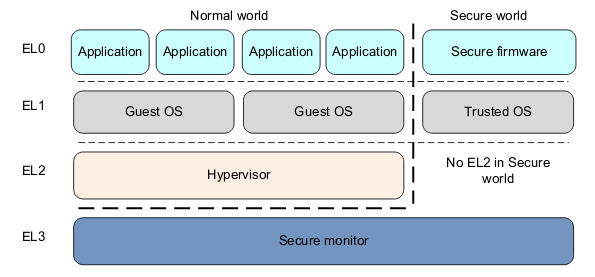
\includegraphics[scale=0.6]{images/tesi7.png}
\caption[ARMv8 Exception Levels]{ARMv8 Exception levels and their main purpose}\label{fig:armv8el}
    \end{center}
\end{figure}

We describe briefly the function of each exception level:
\begin{itemize}
    \item \textbf{EL0} is the lowest exception level, often referred to as ``unprivileged''
        in opposition to every other, ``privileged'', level. It has severe 
        limitation in accessing system registers and failure to respect them
        is met with a synchronous abort exception. It is meant to run user applications, 
        processes below the kernel.
    \item \textbf{EL1} is the first privileged level. It is where most interrupts end
        up and is meant for the OS kernel.
    \item \textbf{EL2} is the Hypervisor level; here resides hardware support for virtualization,
        a level meant to supervise virtual machines. For example, KVM is an in-kernel
        virtualization running at level \textbf{EL2} and supervising the virtual kernel 
        at \textbf{EL1}.
    \item \textbf{EL3} is used to separate the system into secure partitions with the
        hardware TrustZone support.
\end{itemize}

\subsection{Changing Exception Level}
A change in the current exception level can be either caused by a willing decision
of a higher privilege \textbf{EL} to a lower privilege \textbf{EL} or following 
an exception. Moreover, an exception cannot be taken to a lower exception level (e.g. if the core 
is currently at \textbf{EL2} and an interrupt line that should be handled
at \textbf{EL1} is asserted it will be ignored as long as the exception
level is not lowered, regardless of interrupt enabling). 
To access a lower exception level an {\tt eret} instruction is required: {\tt eret}
loads the state stored in \textbf{SPSR\_ELn} (see \ref{spsr}), where \textbf{ELn} 
is the current exception level, as the new system status (exception level included).
Since no exception is ever handled at \textbf{EL0}, \textbf{EL0} is only reachable 
through {\tt eret} instructions.

Exceptions are normally taken to \textbf{EL1} but can be set to run in \textbf{EL2}
or even \textbf{EL3} by configuring corresponding system registers \textbf{HCR\_EL2}
and \textbf{SCR\_EL3}, called \textit{Hypervisor Configuration Register} and \textit{Secure Configuration}
Register respectively. 

It is also possible to change execution \textit{state} (i.e. AArch64 or AArch32)
during runtime but that is irrelevant for the scope of this work, as it lies
entirely in AArch64.

\section{Registers}
\subsection{General Purpose Registers}
One of the immediate benefits of a 64-bits architecture is a larger register pool:
ARMv8 uses 31 64-bits wide general purpose registers, more than doubling from
ARMv7.
The registers are numbered from \textbf{x0} to \textbf{x30}. Although they are
freely accessible the developer should be mindful of their secondary purpose
for function calling convention (both C and Assembler):
\begin{itemize}
    \item \textbf{x0} to \textbf{x7} are used to hold both arguments and return
        value (only \textbf{x0}) of a C function.
    \item \textbf{x8} is used to pass an indirect result value (e.g. a returned 
        structure, in which case x8 holds the address to a properly set memory
        location).
    \item \textbf{x9} to \textbf{x18} are used to hold local variables in a 
        routine call. They are caller-saved, which means that it is the caller
        responsibility to preserve their content before issuing a C function call.
    \item \textbf{x19} to \textbf{x28} are similar temporary registers, but for 
        the callee to restore before returning; they are referred as callee-saved.
    \item \textbf{x29} is the frame pointer.
    \item \textbf{x30} is the link register.
\end{itemize}
Every general purpose register also has a 32 bit alias obtained replacing ``x''
with ``w'' in the register's name (from \textbf{w0} to \textbf{w30}) that permits
access to the lower (i.e. least significant) 32 bits of the register; the upper 
32 bits are ignored.

\begin{figure}[h]
    \begin{center}
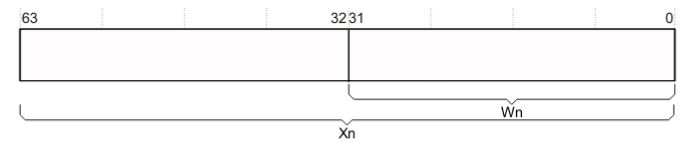
\includegraphics[scale=0.55]{images/tesi8.png}
\caption[32 bit alias]{64 bit register with ``x'' and ``w'' access}\label{fig:32reg}
    \end{center}
\end{figure}

\subsection{Special Registers}
\label{spsr}
There are 5 special registers:
\begin{description}
    \item[Zero Register:] \textbf{xzr} and \textbf{wzr} provide access (as 64 and
        32 bits register respectively) to a special register that ignores write
        attempts and always read as zero.
    \item[Program Counter (pc):] up until ARMv7 the program counter was a general purpose
        register held in \textbf{r15}. In ARMv8 it has a very limited access,
        being read only and only implicitly used in certain instructions. This is 
        one of the biggest differences with previous architecture and caused a 
        lot of initial confusion; its restrictiveness results nonetheless in a
        much clearer and less error prone program flow.
    \item[Exception Link Register (elr):] without free access to the program counter
        the system must provide an alternative way to restore a process' execution
        point. The exception link register holds the exception return address: it 
        is automatically filled when one is fired and can be overwritten. Upon
        executing an {\tt eret} instruction the value in \textbf{elr} is set as the
        program counter.
    \item[Saved Process Status Register (spsr):] similarly to \textbf{elr}, this
        register is automatically initialized with various status informations
        upon taking an exception, and is restored (after eventual modification)
        with an {\tt eret} instruction.
    \item[Stack Pointer (sp):] The current stack pointer. It is freely accessible
        both in read and write operations.
\end{description}

\begin{figure}[t]
    \begin{center}
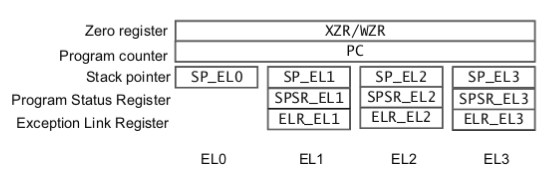
\includegraphics[scale=0.68]{images/tesi9.png}
\caption[special registers]{AArch64 Special Registers}\label{fig:specialreg}
    \end{center}
\end{figure}

As depicted in figure \ref{fig:specialreg} some special registers have different
versions for different exception levels: there is a separated stack pointer 
for all four of them and \textbf{EL0} is the only level missing \textbf{spsr}
and \textbf{elr} (owing to the fact that they are exception related registers, and
\textbf{EL0} never deals with exceptions or {\tt eret} instructions).

Access to a special register from a different exception level is permitted if 
said register belongs to a lower level: for example \textbf{EL3} can set all the
other stack pointers (including its own), but \textbf{EL1} trying 
to do the same will trigger an abort for \textbf{sp\_el2} and \textbf{sp\_el3}.

\subsection{System Registers}
Another significant turn from ARMv7 is the absence of a coprocessor interface.
A coprocessor is an auxiliary core used to supplement the functions of the primary
processor; ARMv7 specified a generic coprocessor interface to connect up to 
15 assisting cores, one of which was reserved for system registers management.
While coprocessors had to be controlled via specific instructions ARMv8 system registers
are directly accessed in Assembler with the {\tt mrs} and {\tt msr} instructions
as per any other register. This is a welcome change that simplifies the developer's
approach to system configuration.

Similarly to special registers many system registers have different, banked versions
for some or all exception levels (usually not \textbf{EL0}), each with the
suffix \textit{\_ELn} to indicate the corresponding level.
These registers are usually 32 bits wide. What follows is a list of system registers
considered most important for the purpose of this work; for a detailed description
of the various bit fields refer to the ARM reference manual \cite{armarm}.
\begin{description}
    \item[Exception Syndrome Register:] \textbf{ESR\_EL\textit{n}}, for each exception 
        level holds the information regarding the last occurred exception (only
        for synchronous and SError, not for IRQs and FIQs. See \ref{exceptions}
        for more on exceptions). It is necessary to distinguish between exception
        classes and to find details specific to the cause of disruption in normal
        program flow.
    \item[Fault Address Register:] \textbf{FAR\_EL\textit{n}}, it is used in pair 
        with \textbf{ESR\_EL\textit{n}} to find which address caused a Data or 
        Instruction synchronous abort.
    \item[Hypervisor Configuration Register:] \textbf{HCR\_EL2}, controls 
    virtualization settings and trapping of exceptions to \textbf{EL2}.
    \item[Memory Attribute Indirection Register:] \textbf{MAIR\_EL\textit{n}}, 
        stores the user-provided memory attribute encodings corresponding to the
        possible values in a MMU translation table entry for translations at level \textit{n}.
    \item[Multiprocessor Affinity Register:] \textbf{MPIDR\_EL1} is the 
        executing core id, used mainly to distinguish on which core the code is 
        running on.
    \item[Secure Configuration Register:] \textbf{SCR\_EL3} controls Secure 
    state and trapping of exceptions to EL3.
    \item[System Control Register:] \textbf{SCTLR\_EL\textit{n}} controls 
    architectural features, for example the MMU, caches and alignment checking.
    \item[Translation Table Base Register 0:] \textbf{TTBR0\_EL\textit{n}}, holds
        the address to the MMU translation table used normally at each exception level.
    \item[Translation Table Base Register 1:] \textbf{TTBR1\_EL1}, holds
        the address to the a special translation table used to separate application
        and kernel space. See section \ref{mmu} for more.
    \item[Vector Based Address Register:] \textbf{VBAR\_EL\textit{n}} is a pointer 
        to the exception vector table for level \textit{n}.
\end{description}

\subsection{PSTATE}
A reader with experience in ARM architecture will surely notice the lack of a
current program status register holding informations like the current exception
level, aritmetic flags, interrupt mask and so on.
The AArch64 version of said register is implicitly present and not directly 
accessible. Instead, the single fields are supplied to read and
write independently; this collection of ``fake registers'' is globally called 
\textbf{PSTATE}; the single fields and their meaning are listed in table \ref{pstatetable}.
 Curiously, querying for the \textbf{CPSR} register in a GDB 
debugger will correctly display the \textbf{PSTATE} components as a whole, although
no such register can be loaded from or stored to even with Assembler instructions.

\begin{table}[t]
    \begin{center}
    \begin{tabular}{|c|c|c|}
    \hline
    \rowcolor[HTML]{9B9B9B} 
    Field name & Register handle              & Description                                                                                                                                                                                           \\ \hline
    N          & \cellcolor[HTML]{FFFFFF}None & Negative condition flag                                                                                                                                                                               \\ \hline
    Z          & None                         & Zero condition flag                                                                                                                                                                                   \\ \hline
    C          & None                         & Carry condition flag                                                                                                                                                                                  \\ \hline
    V          & None                         & Overflow condition flag                                                                                                                                                                               \\ \hline
    D          & daifset and daifclr          & Debug mask bit                                                                                                                                                                                        \\ \hline
    A          & daifset and daifclr          & SError mask bit                                                                                                                                                                                       \\ \hline
    I          & daifset and daifclr          & Interrupt mask bit                                                                                                                                                                                    \\ \hline
    F          & daifset and daifclr          & Fast interrupt mask bit                                                                                                                                                                               \\ \hline
    SS         & None                         & Software Step bit                                                                                                                                                                                     \\ \hline
    EL         & CurrentEl                    & Current exception level                                                                                                                                                                               \\ \hline
    nRW        & None                         & \begin{tabular}[c]{@{}c@{}}Current execution state\\ (AArch32 or AArch64)\end{tabular}                                                                                                                \\ \hline
    SP         & None                         & \begin{tabular}[c]{@{}c@{}}Stack pointer selector\end{tabular} \\ \hline
    \end{tabular}
    \label{pstatetable}
    \caption[PSTATE fields]{PSTATE fields definitions}
\end{center}
    \end{table}

\section{Exception Handling}
\label{exceptions}
In ARM architecture exceptions are conditions or system events that require some 
action by privileged software to ensure smooth 
functioning of the system; said condition is taken care of immediately by interrupting
the normal flow of software execution and starting another routine (the exception
handler).
There are several classes of exceptions; every class can branch in different kinds,
and every exception can be either synchronous or asynchronous (see figure \ref{fig:exceptions}).

The code to run when an exception is fired is specified by the developer in an 
exception vector table. The pointer to the exception vector table is written to 
the \textbf{VBAR\_EL\textit{n}} register, with \textit{n} ranging from level 1 to 3,
so every exception level has its own table (nothing prevents multiple levels
to point to the same table however). For exceptions fired while at \textbf{EL0} 
the table for \textbf{EL1} is referenced.

The exception table can be anywhere in memory but must be 128 bytes aligned and 
must have the format specified in table \ref{etable}.
Each entry in the table is 16 instructions long, allowing for some control logic 
to be present in the top level handler as well before branching to a more complex
routine.
The table can be divided in four sections:
\begin{enumerate}
    \item handlers to be used when the exception does not change neither the current 
        exception level nor the stack pointer.
    \item handlers to be used when the exception does not change the current 
        exception level but should use a specific stack pointer.
    \item handlers to be used when the exception elevates the privilege level and
        the execution state is in AArch64.
    \item handlers to be used when the exception elevates the privilege level and
        the execution state is in AArch32.
\end{enumerate}

Each section has four different handlers for synchronous exceptions, IRQ, FIQ
and SError. The Stack Pointer to be loaded is chosen by the stack pointer selector
field in the current state register (see table \ref{pstatetable}); it can either be the current stack pointer or 
a memory address banked for the destination level.

\begin{table}[t]
    \begin{center}
    \begin{tabular}{|l|l|l|}
    \hline
    \rowcolor[HTML]{9B9B9B} 
    Address           & Exception type & Context                                                                            \\ \hline
    VBAR\_ELn + 0x00  & Synchronous    &                                                                                    \\ \cline{1-2}
    VBAR\_ELn + 0x80  & IRQ/vIRQ       &                                                                                    \\ \cline{1-2}
    VBAR\_ELn + 0x100 & FIQ/vFIQ       &                                                                                    \\ \cline{1-2}
    VBAR\_ELn + 0x180 & SError/vSError & \multirow{-4}{*}{\begin{tabular}[c]{@{}l@{}}Current EL\\ with SP0\end{tabular}}    \\ \hline
    VBAR\_ELn + 0x200 & Synchronous    &                                                                                    \\ \cline{1-2}
    VBAR\_ELn + 0x280 & IRQ/vIRQ       &                                                                                    \\ \cline{1-2}
    VBAR\_ELn + 0x300 & FIQ/vFIQ       &                                                                                    \\ \cline{1-2}
    VBAR\_ELn + 0x380 & SError/vSError & \multirow{-4}{*}{\begin{tabular}[c]{@{}l@{}}Current EL\\ with SPx\end{tabular}}    \\ \hline
    VBAR\_ELn + 0x400 & Synchronous    &                                                                                    \\ \cline{1-2}
    VBAR\_ELn + 0x480 & IRQ/vIRQ       &                                                                                    \\ \cline{1-2}
    VBAR\_ELn + 0x500 & FIQ/vFIQ       &                                                                                    \\ \cline{1-2}
    VBAR\_ELn + 0x580 & SError/vSError & \multirow{-4}{*}{\begin{tabular}[c]{@{}l@{}}Lower EL\\ using AArch64\end{tabular}} \\ \hline
    VBAR\_ELn + 0x600 & Synchronous    &                                                                                    \\ \cline{1-2}
    VBAR\_ELn + 0x680 & IRQ/vIRQ       &                                                                                    \\ \cline{1-2}
    VBAR\_ELn + 0x700 & FIQ/vFIQ       &                                                                                    \\ \cline{1-2}
    VBAR\_ELn + 0x780 & SError/vSError & \multirow{-4}{*}{\begin{tabular}[c]{@{}l@{}}Lower EL\\ using AArch32\end{tabular}} \\ \hline
    \end{tabular}
    \caption[Exception Table]{Exception table format.}
    \label{etable}
\end{center}
    \end{table}

\subsection{Interrupts}
Interrupts can be fast interrupts (FIQ) or normal interrupts (IRQ). Aside from the fact 
that FIQ have higher priority these two types of exception are virtually identical,
and fast interrupts are considered a vestige from past architectures.\\
Usually it is the developer's responsibility to route an interrupt source to 
IRQ or FIQ.
Interrupts are tipically associated with external hardware and connected via 
input pins to the processor; The connection can be direct or, more commonly, pass through
an external device called interrupt controller that elaborates interrupt priorities
and organization (see section \ref{gic}).

Because the occurrence of interrupts is not directly related to the instruction
cycle being executed by the core at any given time, they are classified as
asynchronous exceptions.

 \begin{figure}[t]
 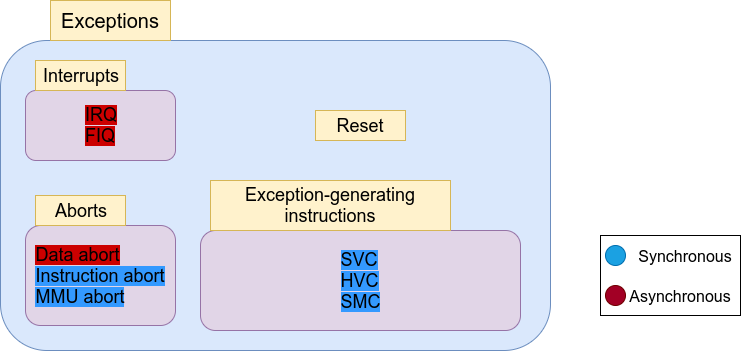
\includegraphics[scale=0.525]{images/tesi10.png} 
 \caption[Exceptions]{Tree of exception classes.}\label{fig:exceptions}
 \end{figure}

\subsection{Aborts}
Abort exceptions, also called system errors (SError), occur every time an abnormal
condition is met during a memory access. Instruction Aborts result from an error
during an instruction fetch cycle, while Data Aborts follow failed data access.

Despite the names depicting error conditions, aborts can work in perfectly normal
and predictable flows. This is the case of MMU faults, generated by the Memory
Management Unit on occasions like access to dirty page entries.
The severity of conditions that set off abort exceptions can be configured to 
some extent with system registers; for example, a TLB miss can be ignored or 
fire an exception, and memory accesses can pass through address alignment 
and permission checks which may or may not interrupt the process.

Aborts can be both synchronous and asynchronous: MMU faults and alignment induced 
aborts are always synchronous, while data aborts can be asynchronous in certain
situations.

\subsection{Reset}
Reset is a special exception, fired on power up of the processor. Its handler is 
implementation-specific and presumably located at address {\tt 0x80000}, the starting
point for the loaded kernel, in the case of BCM2837.

\subsection{Exception Generating Instructions}
We have seen that a core can lower its exception level with {\tt eret}, but can
only increase it through an exception. For this purpose there are Assembler instructions
that induce an exception to a higher execution level, usually to require a service 
paired with a higher privilege. The most obvious example of this behaviour are
system calls.
\begin{itemize}
    \item \textbf{SVC:} the \textit{supervisor call} instruction fires an exception
        handled at \textbf{EL1}. Used by user programs to require kernel services.
    \item \textbf{HVC:} the \textit{hypervisor call} instruction fires an exception
        handled at \textbf{EL2}. Used by the guest OS to require hypervisor services.
    \item \textbf{SMC:} the \textit{secure monitor call} instruction fires an exception
        handled at \textbf{EL3}. Used to require \textit{secure world} context
        switch.
\end{itemize}
Since those exceptions follow an instruction execution they are by definition
synchronous.

\section{Caches}
\label{cache}
A cache is a block of memory with faster access than the memory normally used.
Whenever the RAM is read the resulting value can be stored in this intermediate,
efficient ephimeral storage unit; future references can then be extracted from 
the cache instead (provided the original memory location was not modified) for
a significant increase in performance.
Since slower is normally cheaper, adding a small amount of high quality memory can
speed up the whole system without having to use an expensive replacement.

The ARMv8 specification defines three different cache levels; the processor can
then implement an arbitrary number of them. The cache levels are distinguished 
based on their position on the route from the single core to the external memory.

 \begin{figure}[t]
 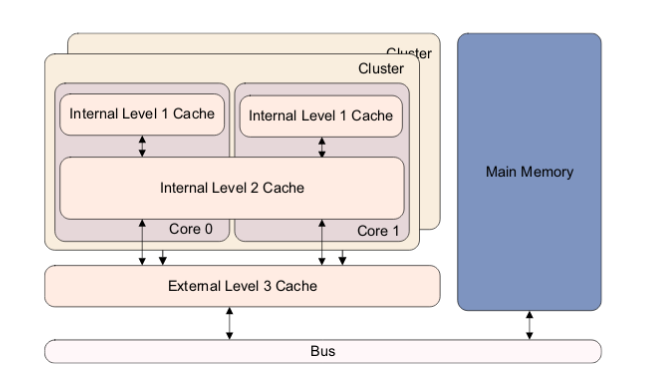
\includegraphics[scale=0.6]{images/tesi12.png} 
 \caption[Cache Levels]{Position of different cache levels in the system.}\label{fig:cache}
 \end{figure}

 In figure \ref{fig:cache} we can see the disposition of the levels. The distance
 from the core issuing a memory access is also an important factor in performance.
When a core requires a memory location, the address is first searched for in 
the level 1 cache, which is core specific and not shared. If nothing is found 
the lookup continues hierarchically to the level 2 cache, which is shared among
cores but internal to the processor. Another miss results in the third cache level,
which is eventually external to the processor.

A specialized device, the cache controller, ensures this search/update mechanism
works smoothly. Care must be taken to avoid problematic coherency situations, where
the content of caches and main memory differ.

Since the objective of this work is to build an educational experience performance
is not a relevant factor; therefore, caches are simply disabled altogether.
Yet a generic understanding of caching is required to correctly setup memory
attributes when configuring the MMU.

\section{Multiprocessor}
Although not mandatory, the ARMv8 architecture is specifically structured to 
host systems with more than one core, like the Cortex-A53 CPU.
In a multicore environment each core has both personal and shared resources:
the registers (general purpose and system) are tipically duplicated and have a
localized effect, while the main memory is shared by all cores at all times.
As seen in the previous section the same applies to caches, with memory banks closer
to the core itself being personal while others are shared.

Each core has its own execution thread, identical or different from 
the others. The A-53 processor has a single clock input, so every core runs at
the same frequency.
% Instruction Level Parallelism?

At a shallow level, the only register one should be concerned with when dealing 
with parallelism is \textbf{MPIDR\_EL\textit{n}}. It contains the identifying number
for both cluster and core that is currently executing, so reading it yields different
results depending of who is doing it. On the A-53 there is only
one cluster and four cores (indexed from 0 to 3).

When the reset interrupt is fired execution starts only for the first core; the
remaning three are held in a waiting state (as if by executing a {\tt WFE} instruction).
They can be woken up by executing a {\tt SEV} (send event) instruction, at which
point execution starts at address {\tt 0x80000} for everyone else.
The most immediate way to split execution into different threads is to check 
\textbf{MPIDR} and follow up with a conditional branch. From there each core should be parked in 
a spinlock, waiting to be released and directed towards the code it should
execute.

\section{ARM Timer}
The Cortex A-53 implements a generic ARM timer interface that can be used for interrupts
and time scheduling. Despite its apparently simple purpose this is a very convoluted
internal device used to virtualize timers for guest OSes as well.
Given such functions are not needed in this work, the explaination will focus 
on the physical counter and interrupt setting registers.

First of all, the timer must be initialized. It has a fixed running frequency
of 62.5 MHz that increments a 64-bits counter on each tick, but by default the 
timer registers cannot be accessed at lower 
exception levels. Setting the proper bits of \textbf{CNTHCTL\_EL2} 
and \textbf{CNTKCTL\_EL1} signal clearance of access from \textbf{EL2} 
and \textbf{EL1} to lower levels, respectively.\\

From there, every exception level (and each core) but \textbf{EL0} have its own timer to configure
and use freely. Additionally, \textbf{EL1} and \textbf{EL2} can benefit from a
virtual timer with a counter value equal to the physical one minus a 
specified offset (register \textbf{CNTVOFF}), for a total of five channels.
Each timer is controlled through four classes of registers:
\begin{itemize}
    \item \textbf{Control:} 32-bits registers named 
        \textbf{CNT\textit{t}\_CTL\_EL\textit{n}}, where \textit{t} represents the
        kind of timer (e.g. \textit{P} for physical, \textit{V} for virtual, 
        \textit{H} for hypervisor) and
        \textit{n} is the exception level. They only use 3 bits to determine whether
        the timer is enabled, if the interrupt should be masked and if the condition
        has been met (i.e. the time alarm has been reached).
    \item \textbf{Counter:} the ever growing 64-bits counter register, 
        named \textbf{CNT\textit{t}CT\_EL\textit{n}}.
    \item \textbf{Compare Value:} \textbf{CNT\textit{t}\_CVAL\_EL\textit{n}}, holds
        the compare value of the corresponding timer. The condition for the timer
        is met when $Counter - CompareValue >= 0$.
    \item \textbf{Timer Value:} \textbf{CNT\textit{t}\_TVAL\_EL\textit{n}}, is a
        convenience 32-bits register for setting the next timer interrupt. On write,
        the compare value is set to the current timer plus the written timer value.
\end{itemize}

The memory mapped generic interrupt controller can be used to decide which kind 
of interrupt (IRQ or FIQ, if any) is fired on condition met. Then, an appropriate
value can be loaded onto the timer value register, and eventually an exception will
be fired. Timer interrupt lines are de-asserted either by setting a new timer
in the future or by disabling the counter altogether.
Even at the same exception level, physical and virtual timers have separate interrupt 
lines. In this project both are used at \textbf{EL1} by the abstraction layer: 
the physical line is routed to normal interrupts while the virtual one is managed
by a FIQ.

\clearpage{\pagestyle{empty}\cleardoublepage}
\chapter{The Memory Management Unit}
\label{mmu}
The Memory Management Unit is a device found in most CPUs tasked with the objective
of translating from virtual memory addressing to physical addressing. The Cortex-A53
is no exception and has an advanced internal MMU. It is such an important component
of the system and of any Operating System that even if it's technically 
part of the ARMv8 specification it deserves a chapter on its own.

The main purpose of address translation is to allow each process to have its own
virtual address space that has nothing to do with how much memory is available 
(and where this memory is located) on the system, with hardware MMIO and other
processes hidden from its view.
If the memory management unit is active any address referenced by a process is first
elaborated and translated: different sections of the 64-bits address (starting
from the most significant) are used to index different levels of a tree containing
translation entries. While translating there can also be additional checks on 
whether the current exception level has the proper permissions to access 
the resulting physical memory. For example memory blocks where the kernel is loaded
should not be accessed in any way by \textbf{EL0} code; in a similar way memory
that is writable at \textbf{EL0} cannot be allowed to execute at higher permission
levels. The latter constriction is built in the specification by default; the former
should instead be enforced by the developer via MMU configuration.\\
Only after translation and permission checks are done the actual memory access 
is performed; however, most of the process is handled by the hardware and 
can be almost entirely ignored by the programmer after the initial setup.

\section{Address Translation}
As briefly mentioned in the introduction, when the MMU is active every address is 
treated as an array of indexes for the translation table. The translation table is 
a tree of translation entries that maps a section of RAM: each level of the 
tree has entries covering a certain number of elements in the next level until the 
last, that corresponds directly to memory.\\

The example that follows considers a tree where each entry before last level
points to 512 more entries and 
depicts a trivial ``identity'' mapping: every virtual address is translated in 
the same physical address. The bottom level covers a 4KiB block of memory directly
(the reason for these numbers will be explained in section \ref{translationsize}). There
are four levels in the tree, level 0 to 3.
Presume we want to translate a 64-bits address:
\begin{itemize}
    \item the 16 most significant bits are reserved for kernel space virtualization
        (more on this topic in section \ref{kernelvirt}).
    \item bits 47:39 are the level 0 table and reference a level 1 entry. Each
        level 0 entry spans a 512 GiB memory range ($2^39$).
    \item bits 38:30 are the level 1 table and reference a level 2 entry. Each
        level 1 entry spans a 1GiB memory range ($2^30$ or $512 GiB / 512$).
    \item bits 29:21 are the level 2 table and reference a level 3 entry. Each
        level 2 entry spans 2 MiB memory range, similarly to previous levels.
    \item bits 20:12 are the level 3 table and reference the last level, made of 
        direct memory blocks. Each memory block is 4KiB wide.
    \item bits 12:0 are the offset for the last memory block and index the actual
        word referenced.
\end{itemize}

 \begin{figure}[h]
 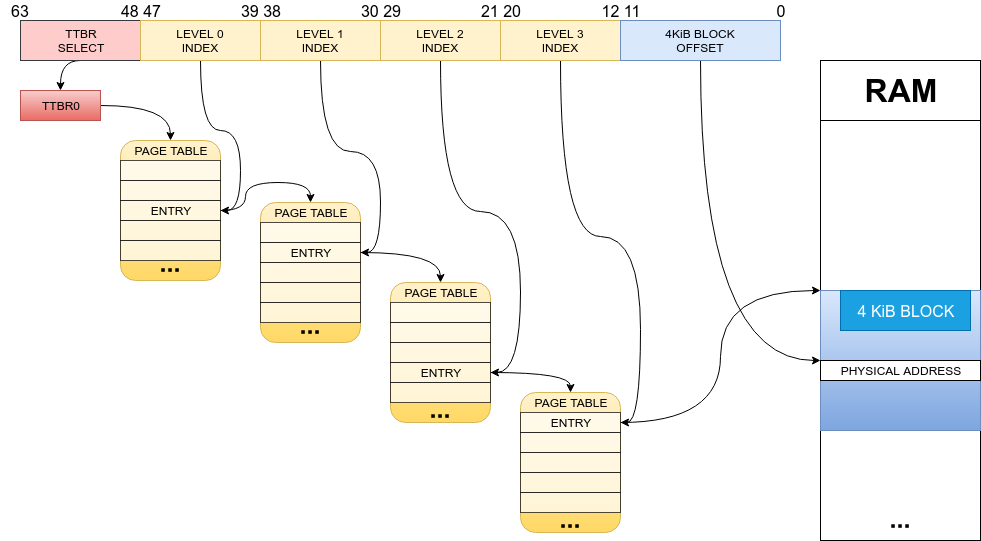
\includegraphics[scale=0.42]{images/tesi15.png} 
 \caption[Address Translation Example]{ Example of the address translation process .}\label{fig:translation}
 \end{figure}


In this mundane example it is evident how the translation process is arbitrary;
every level can simply be cut off and the resulting address be obtained by adding
the intermediate indexes and the remaining bits (to be considered as the final 
offset).\\
This is not possible anymore if the translation function is not an identity,
in which case the translation function is codified by the pointers in the table entries;
the table entry marks the beginning of the next level of tables and the corresponding
piece of virtual address indexes the chosen entry.

\subsection{Granule Size}
\label{translationsize}
With granule size we refer to the smallest possible block of memory that can be 
indexed by the MMU tables; in the previous example, 4KiB.
The ARMv8 specification allows for three different granule sizes: 4KiB, 16KiB and 64KiB.
The actual ARM processor abiding to the standard can in turn implement those granules
only partially, and fortunately the Cortex-A53 implements them all.
The granule size is a global setting, affecting the entirety of the page table.
Different granule size dictate how many levels is possible to have and how many
entries are in each table (for example, a granule of 64 KiB allow only 3 levels
and a granule of 16KiB will result in 10-bits wide address sections).

A small granule size will result in more control but also in a bigger table; to 
divide a 2GiB RAM into 4KiB blocks an Operating System will need 524288 64-bits
wide table entries, for a total of 4MiB of allocated memory.
Choosing a fine grained control does not mean commiting to it, however. If there
are large sections of memory with the same memory attributes and virtual addressing
(e.g. MMIO memory that should generally not be accessed by user processes) the 
developer can ``cut early'' the page table tree and use any intermediate memory
range. In the above example we could arbitrarily stop at level 2 and create a part
of the table with direct entries spanning 2 MiB each, situation photographed in
figure \ref{fig:translation2}.

 \begin{figure}[h]
 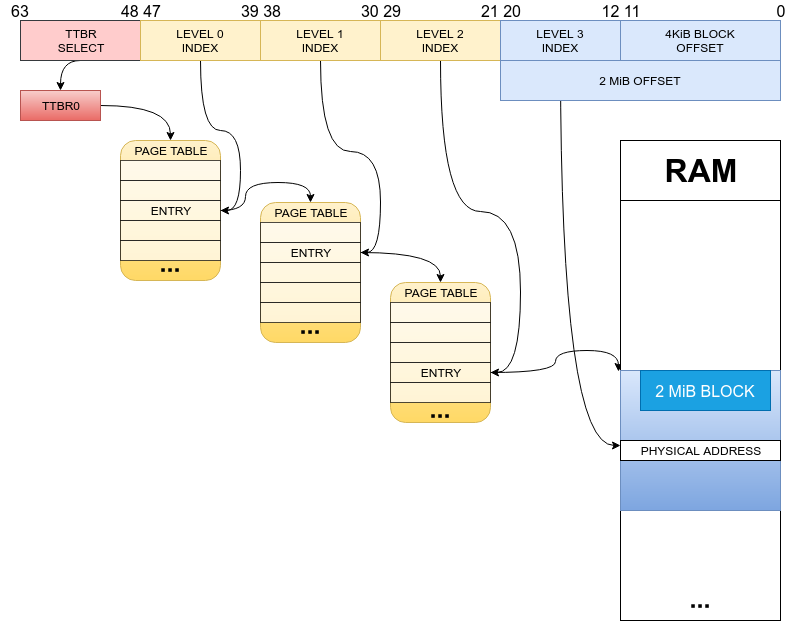
\includegraphics[scale=0.48]{images/tesi16.png} 
 \caption[Address Translation Example]{ Here the last 21 bits are
 used as a bigger offset for a 2 MiB block of memory}\label{fig:translation2}
 \end{figure}

\section{Table Descriptor Format}
When in AArch64 there is a single accepted format for table entries. We will now
consider the configuration consequential to a 4 KiB granule size; other choices
differ sligtly in translation indexes width and position, but maintain the same
core concepts. The table descriptor is 64-bits wide, separated in differently sized
 fields.

Any table entry is one of two types:
\begin{enumerate}
    \item \textbf{A table descriptor} that points to another table entry in the 
        next level.
    \item \textbf{A block entry} that resolves directly into a memory range of 
        variable size, depending on the level.
\end{enumerate}

The entry type is defined by the two least significant bits in the descriptor, 
as depicted in table \ref{tab:desc}; an invalid entry leads to an MMU fault exception.
Note that not every level can host a block entry; with a granule size of 4 KiB, 
level 0 does not admit that kind of descriptor.

\begin{table}[]
    \begin{center}
    \begin{tabular}{|c|l|}
    \hline
    \rowcolor[HTML]{9B9B9B} 
    \begin{tabular}[c]{@{}c@{}}Entry Type\\ field\end{tabular} & Meaning          \\ \hline
    00                                                         & Invalid          \\ \hline
    01                                                         & Block Entry      \\ \hline
    10                                                         & Invalid          \\ \hline
    11                                                         & Table Descriptor \\ \hline
    \end{tabular}
    \label{tab:desc}
    \caption[Page Entry Types]{Page entry types.}
\end{center}
    \end{table}

\subsection{Table Descriptors}
Table descriptors point to a table entry in the next level. Bit fields have the 
following meaning:
\begin{itemize}
    \item \textbf{[0]} marks the validity of the entry; 1 is valid, 0 is invalid.
    \item \textbf{[1]} is the entry type. It is 1 for table next level descriptors.
    \item \textbf{[2:11]} are ignored/reserved bits.
    \item \textbf{[12\footnote{\label{4knote} This value can be different for granule
        sizes other than 4KiB}:47]} is the address of the next level table. It is codified
        as if it started from the least significant bit, with 
        [11\footnote{see footnote \ref{4knote}}:0] bits assumed
        as 0. Because of this all page tables must be 4096 ($2^{12}$) bytes aligned.
    \item \textbf{[48:58]} are ignored/reserved bits.
    \item \textbf{[59]} PXNTable field: \textit{private execute never} bit for subsequent
        levels of lookup; if set the memory range covered by this and following entries
        cannot be executed by code at level \textbf{EL0}.
    \item \textbf{[60]} XNTable field: \textit{execute never} bit for subsequent levels
        of lookup; if set the memory range covered by this and following entries
        cannot be executed.
    \item \textbf{[61:62]} APTable field: \textit{access permission} bits for subsequent levels
        of lookup; this field enforces permission rules for the memory range
        indexed by this and following entries, combined in a hierarchical 
        fashion (see table \ref{tab:aptable}). Subsequent table entries can
        further restrict the permission rules but cannot loosen them; failure
        to heed said rules will result in an appropriate abort exception.
    \item \textbf{[63]} NSTable field: when in secure state this bit specifies
        the security state for subsequent levels of lookup. When not in secure state
        it is ignored.
\end{itemize}

\begin{table}[h]
    \begin{center}
    \begin{tabular}{|c|l|}
    \hline
    \rowcolor[HTML]{9B9B9B} 
    \multicolumn{1}{|l|}{\cellcolor[HTML]{9B9B9B}APTable{[}1:0{]}} & Restriction                                                                                                                                            \\ \hline
    00                                                             & No effect on subsequent levels of lookup                                                                                                               \\ \hline
    01                                                             & \begin{tabular}[c]{@{}l@{}}Any access to this memory range from EL0\\ is forbidden.\end{tabular}                                                       \\ \hline
    10                                                             & Memory is read-only.                                                                                                                                   \\ \hline
    11                                                             & \begin{tabular}[c]{@{}l@{}}Any access to this memory range from EL0\\ is forbidden, while it is read-only for\\  higher privilege levels.\end{tabular} \\ \hline
    \end{tabular}
    \label{tab:aptable}
    \caption[APTable]{Access Permission Table bit fiels. The two bits can be 
    separated and seen as read-only bit ([0]) and \textbf{EL0} access ([1])}
\end{center}
\end{table}

%TODO: immagine fig:desc1

\subsection{Block Descriptors}
\label{mmublock}
Block descriptors represent direct access to a block of memory; when one is reached,
it is the last stage of the translation process. They contain the following bit
fields:
\begin{itemize}
    \item \textbf{[0]} marks the validity of the entry; 1 is valid, 0 is invalid.
    \item \textbf{[1]} is the entry type. It is 0 for block descriptors.
    \item \textbf{[2:4]} memory attributes index field. The value found here
        indexes a memory address configuration defined in corresponding 
        the \textbf{MAIR\_EL\textit{n}} register (see section \ref{mair}).
    \item \textbf{[5]} is the non-secure bit. For memory accesses from 
        secure state specifies whether the output address is in
        the secure or non-secure address map. For accesses from non-secure state
        this bit is ignored.
    \item \textbf{[6:7]} are data access permission bits. Similar to APTable bits,
        they are referred to the immediate block of memory (and can be further
        restricted by previous APTable settings). For possible values see table
        \ref{tab:apbits}.
    \item \textbf{[8:9]} sets the shareability of the memory block, configuring
        caching capabilities.
    \item \textbf{[10]} is the access flag (AF). If it is not set it means the 
        selected entry is accessed for the first time, in which case an MMU abort
        will be fired. The exception handler should take care of the initialization,
        set the access flag to 1 and attempt again the memory access.
    \item \textbf{[11]} is the not global bit (\textit{nG}). If a lookup using this 
        descriptor is cached in a TLB, determines whether the TLB
        entry applies to all ASID values or only to the current ASID value
        (see section \ref{tlb} for more).
    \item \textbf{[12:47]} is the address to the memory block that is pointed by
        the descriptor. It is aligned similarly to the address in a table descriptor,
        but it contains actual memory instead of a next level page table.
    \item \textbf{[48:50]} are ignored/reserved bits.
    \item \textbf{[51]} is the Dirty Bit Modifier (DBM); it is used to keep
        track of differences between caches and real memory. If it is set, caches
        should be checked for stale entries. It can be managed either via 
        hardware or software.
    \item \textbf{[52]} is the Contigous bit, a hint bit indicating that the 
        translation table entry is one of a contiguous set or entries and may be
        be cached in a single TLB entry.
    \item \textbf{[53]} PXN bit: \textit{privileged execute never} bit. If set, the memory block's 
        execution at unprivileged exception levels (\textbf{EL0}) is forbidden.
    \item \textbf{[54]} XN bit: \textit{execute never} bit. If set, the memory block's 
        execution is forbidden.
    \item \textbf{[55:63]} are ignored/reserved bits.
\end{itemize}

\begin{table}[]
    \begin{center}
    \begin{tabular}{|l|l|l|}
    \hline
    \rowcolor[HTML]{9B9B9B} 
    AP{[}2:1{]} & Access from privileged EL & Access from EL0 \\ \hline
    00          & Read and write            & Forbidden       \\ \hline
    01          & Read and write            & Read and write  \\ \hline
    10          & Read-only                 & Forbidden       \\ \hline
    11          & Read-only                 & Read-only       \\ \hline
    \end{tabular}
    \caption[APBits]{Access Permission Bits values. similarly to \ref{tab:aptable},
    the two bits 1 and 0 can be interpreted separately as write restriction for higher
    exception level and access for \textbf{EL0}, respectively.}
    \label{tab:apbits}
\end{center}
    \end{table}

%TODO: immagine fig:desc2


\section{Memory Types and Attributes}
\label{mair}
As previously mentioned the block and table descriptors contain information about
what kind of memory they point to.
Every memory address is one of two possible types: normal or device.
Normal memory is the one used for most memory regions and where there can be 
the most invasive optimizations. Normal memory can be heavily cached and is 
considered to be weakly ordered: the actual number, time and order of access can 
differ from the logical flow of the program without causing semantic errors.

Device memory is used instead for memory mapped peripherals. When the subject is
a device register the order of operations and even repeating the same instruction
might yield unexpected side effects; caching must be disabled too, as the content
of a device bus is often non deterministic.\\
Other than the memory type there are fine tuned attributes to distinguish
what levels of caching and optimization are allowed.

\subsection{Shareability}
In a multiprocessor system the main memory is obviously shared among all the cores.
This can lead to coherency problems in caches external to the individual core (level 2
and level 3, see section \ref{cache}). Hinting who is going to use a certain memory
block can greatly help the system when managing caches, improving performance
and energy cost. There are three possible
shareability options:
\begin{description}
    \item[Non-Shareable:] memory marked as non shareable is assumed to belong to
        a single actor, thus synchronization of access from different cores is 
        not needed.
    \item[Inner Shareable:] this memory can be shared inside the processor (i.e. 
        between the cores) but not outside of it (i.e. in the rest of the system).
    \item[Outer Shareable:] an outer shareable domain is publicly available for 
        every actor in the system and needs to be synchronized on each access.
\end{description}
The shareability attribute is found in the specific field of the block entry descriptor
(see section \ref{mmublock})

\newpage

\subsection{Cache policies}
When a cache search misses and the entry is not found, the respective cache entry is 
updated with the value found on RAM. When the search is successful and the
operation is a write, deciding what location to update is not trivial. \\
Regarding normal memory, the OS developer can specify cache policies as any combination
of the following three classes:

\begin{enumerate}
    \item \textbf{Cacheability:} Non-Cacheable, Inner Cacheable or Outer Cacheable.
    \item \textbf{Update policy:} Write Back or Write Through.
    \item \textbf{Transient:} Transient or Non-Transient
\end{enumerate}

Different cacheability options refer to which fast memory block should be used
- internal to the core, internal to the cluster or external - and were described
 in section \ref{cache}.\\
When \textit{write back} memory locations are updated only the  cache entry
is modified and marked as dirty; corresponding main memory locations are updated 
only when the cache line is evicted or explicitly cleaned.
\textit{Write through} is instead a safer (but slower) approach, where an update 
changes both the cache and the system memory.\\
\textit{Transience} is an hint to the cache controller about how long an address should be 
kept in cache for. This behaviour is implementation defined, not configurable
by the developer.\\

Device memory is treated differently, and thus possesses its own set of attributes:
\begin{enumerate}
    \item \textbf{Gathering:} this property determines whether multiple accesses
        can be merged into a single bus transaction for this memory region. If 
        the address is marked as \textit{gathering} the processor can, for example, 
        merge two byte writes into a single-word half write.
    \item \textbf{Reordering:} attribute defining whether accesses to the same 
        device can be re-ordered with respect to each other. If the address is 
        marked as \textit{non Re-ordering} then accesses within the same block 
        always appear on the bus in the order specified by the code, while
        \textit{Re-ordering} ranges of memory will be subject to read and write
        chains optimization.
    \item \textbf{Early Write Acknowledgement:} identified as \textit{E} 
        or \textit{nE}, declares if an 
        intermediate write buffer between the processor and
        the slave device being accessed is allowed to send an 
        acknowledgement of a write completion. It is only used for closely 
        intertwined operation with special peripherals.
\end{enumerate}

Refer to the Architectural Reference Manual \cite{armarm} for the exact values
and codes of the memory attributes combinations.

\subsection{MAIR Configuration}
Due to the high number of possible combinations (many of which are problably 
scarcely used), the memory attributes 
configuration procedure follows a peculiar and somewhat unconventional approach.
Instead of having separate
fields in the already filled block descriptor format, the programmer defines
up to eight memory attribute combinations codified with 8 bits each which are 
then pushed into the \textbf{MAIR\_EL\textit{n}} register as if in an array.
The block descriptor in turn has a 3-bits field, the memory attribute index,
 that indexes which configuration to use in said array, in a two step process.

 In the image example, the \textbf{MAIR} register is populated with two options
 for cached and non-cached normal memory in the first two bytes. Page table entries
 will then select a combination using the memory attribute index.
 Note that any combination can be placed anywhere in the register and it does not
 need to be correctly initialized in all the eight bytes, as long as only correct
 entries are indexed by the page table.

 \begin{figure}[h]
    \begin{center}
 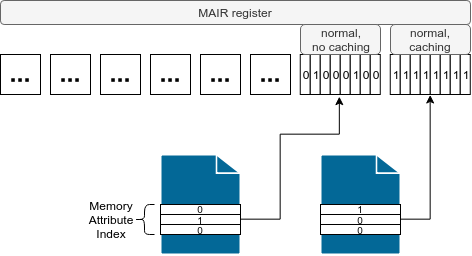
\includegraphics[scale=0.7]{images/tesi17.png} 
 \caption[MAIR Register]{MAIR register configuration and indexing by the page
 table entries.}\label{fig:mair}
    \end{center}
 \end{figure}
 %16 ExbiByte

\section{Kernel Space Virtualization}
\label{kernelvirt}
In a tipical OS environment multiple processes run concurrently and use dynamically
allocated memory and resources. The memory management unit serves to this purpose:
every process has its own set of translation tables managed by the kernel and sees a 
contiguous range of memory at its disposal while in truth it is loaded somewhere
in main memory - maybe not even adjacent or complete.\\
 In this multitude of actors we can
consider the kernel as a process in its own right - albeit of a superior kind -
and because it has no peers and often uses a static memory space the 
translation mechanism is meaningless, if not cumbersome.

To fix this situation the ARMv8 provides a number of features. One may intuitively
imagine different page table references for each Exception Level, but this is 
only partially the case. \textbf{EL0} and \textbf{EL1}, the main levels of operation
for user processes and kernel, share in fact the same two page table registers:
the one assigned to ``normal'' operation, \textbf{TTBR0\_EL1}, and the register
 actually in charge to properly divide user and kernel pages,
 The former is used to translate addresses in the vast majority of the
 immense 64-bits addressing space, holding the base address of the page table
 constructed by the developer; \textbf{TTBR1\_EL1}, the latter, works in the
 same way but is only selected when the 16 most significant bits of the address
 under scrutiny are set to 1, forming a location absurdely far away for any memory 
 bank designed in the foreseeable future.

 The kernel can then operate in this mock memory range with a personal page
 table (possibly as an identity transformation) while normal processes live in 
 lower scope of virtual memory. To accomodate the kernel in this inexistent
 range the addresses in its code must be set properly. This would require either
 a linker script instructing to compile for memory starting at 
 {\tt 0xFFFF00000000000000} (in which case the MMU must be configured and 
 enabled immediately) or compiling the code for relative branch instructions only.
 The latter approach is considered easier as it works even if the MMU is disabled
 and only requires the kernel entry point (the exception table) to be tweaked 
 when address translation is eventually turned on.\\

 As a side note, the condition to select the \textbf{TTBR1\_EL1} register can
 be limited to the second most significant byte of the address set to {\tt 0xFF};
 the first byte can then be freely used by the kernel software for personal 
 purposes.

 \begin{figure}[h]
 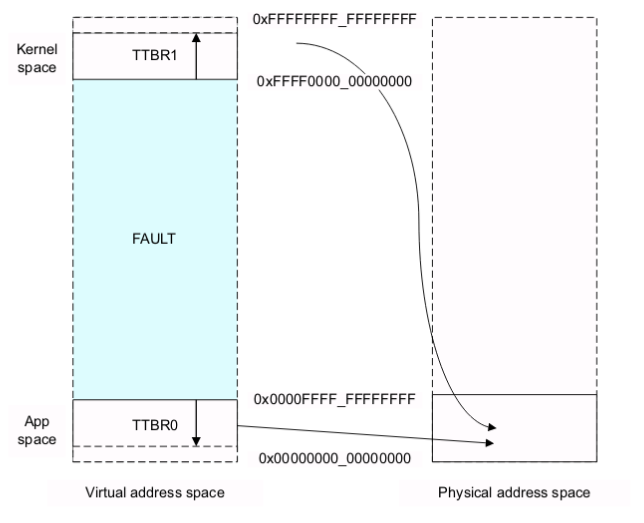
\includegraphics[scale=0.6]{images/tesi11.png} 
 \caption[Kernel memory virtualization]{In this image kernel and user spaces 
 are positioned at the opposites of the address range but both are mapped in 
 the same physical area.}\label{fig:rammap}
 \end{figure}
 %16 ExbiByte


 An example use case might be in support of object-oriented programming languages:
 as well as having a pointer to an object, it might be necessary to keep a 
reference count that keeps track of the number of references, pointers or handles
 that refer to the object, for example, so that automatic garbage collection 
 code can deallocate objects that are no longer referenced. This reference 
 count can be stored as part of the tagged address rather than in a separate table, 
speeding up the process of creating and destroying objects.

\subsection{EL2 and EL3 Translation Process}
Virtualization and secure exception levels have their own page tables. Since they act
as overlay for one or more guest operating systems when enabled there are two translation
stages: the first one is performed by the OS, using \textbf{TTBR\textit{n}\_EL1}
as already explained; the result from this stage is then fed to a second stage,
with tables found in \textbf{TTBR0\_EL2} and \textbf{TTBR0\_EL3}.

Such complex tools are out of the scope of this work.


\section{Translation Lookaside Buffer}
\label{tlb}
The Translation Lookaside Buffer (or TLB) is simply cached memory for address translation
results: when a virtual address is to be translated the TLB is checked first;
if the address is found (TLB hit) then the cached value is used. If not (TLB miss)
a page table walk is performed and the result is stored in the TLB. Alternately,
an MMU fault can be configured to fire.

The TLB and MMU intertwined operation works very differently in ARM compared to 
MIPSEL architecture and with an arguably easier approach for a novice. The TLB 
component activity is almost invisible to the OS developer not caring for 
particular performance optimizations, so it can be safely ignored. The only 
essential part is the configuration of proper page tables for each process.

\subsection{Trivial Approach}
Once the MMU is activated and page tables are initialized the kernel must make 
sure every process can only see its virtual memory share during its designated
time slice. This can be achieved by creating a different page table per process
and simply substituting it completely every time there is a context switch.
A problem presents when a process asks for the same virtual address, that should
however be translated in a different physical address, of one of its peers; 
we shall call them process \textit{a} and \textit{b}.
If the entry relative to \textit{a} is found in the TLB by \textit{b} its value
will be returned without performing a page table walk, and will result in the
wrong memory being accessed.

Without delving too deeply into MMU operation, a simple solution will be to 
flush the TLB cache every time there is a context switch. This will effectively
deny most of the optimization brought by the cache, but will also prevent
incorrect translations.

\subsection{ASID Approach}
A more elegant and efficient solution consists in using an Address Space ID (ASID)
to keep track of process property in TLB entries. The ASID is arbitrarily assigned
to processes by the kernel and stored in the two most significant bytes of either
\textbf{TTBR0\_EL1} or \textbf{TTBR1\_EL1}
When the non-global (\textit{nG}) field of a block entry in the page table is 
set the current ASID is saved alongside the address in a TLB entry. Subsequent
lookups for that address in the TLB cache only match if both the address and the
saved ASID correspond to present values.

% TODO: remember ttbcr; eventually describe MMU register configuration in greater
% detail


\clearpage{\pagestyle{empty}\cleardoublepage}
\chapter{Overview of the BCM2837}
The BCM2837 is the System-on-Chip produced by Broadcom that is used for most
of the Raspberry Pi family of boards, and for the third version specifically.
 Some of them are built with variants like BCM2836 (for the Raspberry Pi 2)
  and BCM2835 (the first used, for the Raspberry Pi 1): the scarce documentation
  is only available for BCM2835 \cite{bcm2835} (and partially for BCM2836 \cite{rev3.4})
  allegedly because nothing changes from the developer perspective; the actual 
  differences have been figured out mostly through reverse engineering from the 
  source code of various Linux distributions.

The BCM2837 contains the following peripherals, accessible by the on-board ARM CPU:
\begin{itemize}
    \item A system timer.
    \item Two interrupt controllers.
    \item A set of GPIOs.
    \item An USB controller.
    \item Two UART serial interfaces.
    \item An external mass media controller (the microSD interface).
    \item Other minor peripherals (I2C, SPI,\ldots).
\end{itemize}

\section{Boot Process}
As is the case for many similar boards the ARM CPU is not the main
actor, but actually more of a coprocessor for the Videocore IV GPU installed
alongside it.

On reset the first code to run is stored in a preprogrammed ROM chip read by the GPU,
called the first-stage bootloader. This first bootloader looks for the first
partition on the microSD card (which has to be formatted as FAT32), mounts
it and loads (if present) a file called {\tt bootcode.bin} from the partition.
This binary is part of the Broadcom proprietary firmware package, and is considered
the second-stage bootloader.\\
At this point of the boot sequence the main memory is still not initialized, so the second-stage
bootloader is run from the L2 memory cache. This firmware initializes the RAM 
and in turn loads on it another file from the microSD card, start.elf.\\
Another firmware for the Videocore, {\tt start.elf} has the responsibility to split 
the RAM in two parts for the GPU and the CPU; after that it reads the config.txt 
file (if present) and loads its parameters starting at address 0x100.
 Finally it does the same with the kernel image and passes control to the ARM CPU.

 \begin{figure}[t]
    \begin{center}
 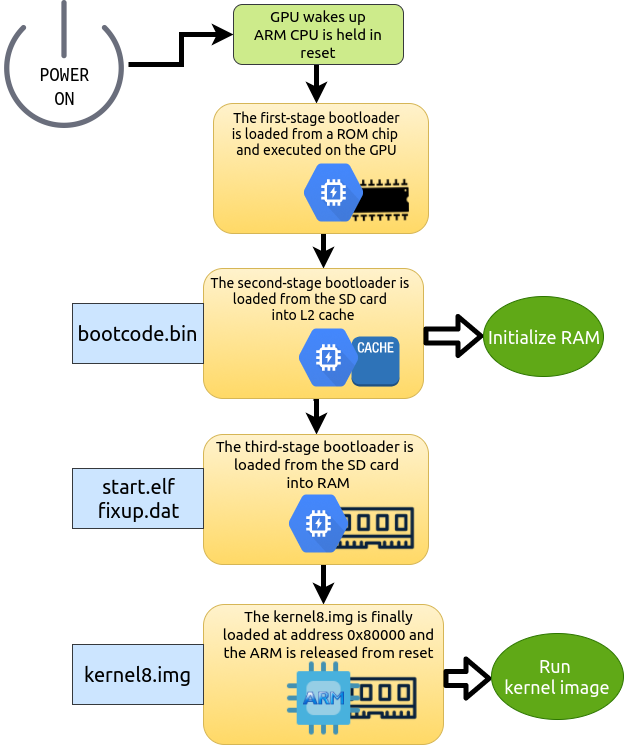
\includegraphics[scale=0.46]{images/tesi1.png}
 \caption[BCM2837 Boot Sequence]{Explanatory diagram on BMC2837 boot sequence}\label{fig:prima}
\end{center}
 \end{figure}
 \clearpage

Every step up until the loading of the kernel image in memory is handled by 
the GPU and can be safely ignored after an initial setup.

\subsection{MicroSD Contents}
The microSD must have its first partition formatted as FAT32; there are no 
further restrictions on following partitions. The absolute bare minimum contents 
are just four files:
\begin{enumerate}
    \item \textbf{bootcode.bin}: second-stage bootloader, necessary for the GPU
            to load the third-stage bootloader.
    \item \textbf{start.elf}: third-stage bootloader, necessary for the GPU to load
            the kernel image into main memory.
    \item \textbf{fixup.dat}: a file containing relocation data to be referenced 
            by {\tt start.elf} when loading into RAM; this allows for the same firmware 
            to be used for all versions of the Raspberry Pi, which range in 
            memory from 256MB to 1GB. If not included the board might still boot,
            but it will likely only report a total of 256MB regardless of the
            actual installed memory banks.
    \item \textbf{kernel8.img}: kernel binary for the ARM CPU.
\end{enumerate}
Of those four files only the kernel image is user provided; the remaining firmware
is distributed and updated in compiled form by the Raspberry Pi foundation with
proprietary licensing from Broadcom.

\subsection{Configuration}
It is possible to configure in different ways the boot process by combining
different firmware binaries and {\tt config.txt} options, but MaldOS always uses
the default with no extra steps needed; this is to ensure the usage is kept
as simple as possible and because the base behaviour never presented any issue.
Of all the available options, only the following two were ever considered 
(but still never implemented).

\subsubsection{Architecture}
The Cortex A-53 can run both ARM32 and ARM64 code. The choice is dictated by the
name of the kernel image: {\tt kernel8.img} makes the CPU start in AArch64 mode,
while {\tt kernel7.img} would start in AArch32. The latter option is preferred.

\subsubsection{Kernel Loading Address}
The GPU loads the kernel image starting at address {\tt 0x80000} in RAM for the
Raspberry Pi 3. By adding a {\tt config.txt} file to the microSD card and using
the {\tt kernel\_address} parameter the image file will be loaded at the specified
starting point. Similarly, by setting the {\tt kernel\_old} parameter to 1 the binary
will be loaded at the beginning of the main memory, at address {\tt 0x0}. This
alias is present for compatibility reasons.

Although these options can bring a more clean memory disposition, it was decided
the advantages were not worth adding an additional file to the necessary setup.
Additionally, while the Raspberry Pi hardware correctly interprets these commands
the Qemu emulated machine is not entirely loyal to reality and actively resists
any attempt to move the kernel to locations other {\tt than 0x80000} (more details can
be found in section \ref{qemu}).

\subsubsection{Memory Split}
As previously mentioned the two main actors on the BCM2837, the quadcode Cortex-A53 ARM
and the Videocore IV GPU, share the same 1GiB RAM space. When not instructed otherwise
the {\tt start.elf} bootloader fixes the separation at address {\tt 0x3C000000}, keeping
64MiB to himself and leaving the rest to the CPU.

This split can be increased in favor of the GPU or minimized even further using
specific {\tt config.txt} parameters. The only graphical feat required by this work
is the display of a simple framebuffer to present textual output; therefore
a reserved memory partition of 64MiB is more than sufficient.
It could be in fact reduced further to 16MiB, but as for the kernel load address 
adding the {\tt config.txt} file was judged unneded effort on the user's side.

\section{Videocore IV}
After the control is passed to the ARM CPU it is never returned to the GPU.
The graphical processor however still has responsibility over some peripherals
and can carry on work under specific requests. The mean of communication 
between the two processing units is the shared RAM memory (and part of the interrupt
controller), specifically under the Mailbox interface.

\subsection{Mailboxes}
Mailboxes are the primary means of communication between the ARM and the 
Videocore firmware running on the GPU. A mailbox is nothing but a memory address
with special access modes tied to an interrupt signal for the receiving end.
Mailboxes consist of one or more 32-bits registers providing status information, read
and write access. If a value is written on the right memory location and the
mailbox is ready to accept data, an interrupt will be fired and the receiver
will have the chance to read the message and act accordingly. The data is 
usually another memory location, whose pointer has been written into the 
actual mailbox, containing arbitrarily long and elaborate parameters.
ARM cores can interrupt each other by using single register mailboxes for inter
processor communication while the relative extra cluster transmission mean have
as many as 9 registers each, although the function of most of them is unknown.
\begin{center}
\begin{table}[h]
    \begin{tabular}{|c|c|}
    \hline
    \rowcolor[HTML]{9B9B9B} 
    Register Name & Function                                                                                                                                        \\ \hline
    read          & \begin{tabular}[c]{@{}c@{}}register to be read for command responses.\\ The 4 least significant bits are the mailbox channel\end{tabular}       \\ \hline
    reserved      & \cellcolor[HTML]{656565}                                                                                                                        \\ \hline
    reserved      & \cellcolor[HTML]{656565}                                                                                                                        \\ \hline
    reserved      & \cellcolor[HTML]{656565}                                                                                                                        \\ \hline
    peek          & \begin{tabular}[c]{@{}c@{}}like the read register but does not remove the \\ value from the message FIFO\end{tabular}                           \\ \hline
    sender        & information about the sender                                                                                                                    \\ \hline
    status        & \begin{tabular}[c]{@{}c@{}}status register, carrying information about the mailbox\\ state (e.g. the message FIFO is empty or full)\end{tabular}\\ \hline
    config        & unknown function                                                                                                                                \\ \hline
    write         & \begin{tabular}[c]{@{}c@{}}register where to write a pointer to the command structure.\\ Adds the message to the GPU's FIFO.\end{tabular}       \\ \hline
    \end{tabular}
    \caption[Mailbox Registers]{CPU-to-GPU mailbox registers list.}
    \end{table}
\end{center}
Regarding the CPU-to-GPU mailbox, additional care must be taken to check whether
the mailbox is full or empty by inspecting the two most significant bits of 
the status register.
After the command has been executed the status register should be polled again
for change and the memory structure passed to the other core will contain the
requested information (if any).
The Videocore accepts lists of multiple commands as messages and organizes
responses in an ordered FIFO that is emptied by reading the mailbox until 
the status register signals there is no more mail.

The data address to be written on the mailbox must be 16 bytes aligned in memory,
as the lowest 4 bits must be overwritten with the so called mailbox channel
number, a parameter detailing the nature of the request. As of time of writing
only two channels are defined: channel 8 for requests from ARM to the Videocore
and channel 9 for requests from the Videocore to the ARM. Apparently, channel 9
exists but has no definied behaviour.


The buffer whose address is written on the mailbox must contain properly structured
data for specific requests. Some of the possible commands from the ARM CPU to the
Videocore include:
\begin{itemize}
    \item Get Broadcom firmware revision number.
    \item Get board model and revision number.
    \item Get board MAC address.
    \item Get current CPU-GPU memory split.
    \item Get or set power state for all the devices on the board.
    \item Get or set clock state for all the devices on the board.
    \item Get on board temperature readings.
    \item Control special GPIOs, like the on board activity led.
    \item Execute code on the Videocore.
    \item Require and manage a framebuffer to be displayed over the HDMI.
\end{itemize}

\begin{table}[b]
    \begin{tabular}{|c|c|}
    \hline
    \rowcolor[HTML]{9B9B9B} 
    Field Size                                                  & Meaning                                                                                                                                        \\ \hline
    32 bits                                                     & buffer size in bytes (including the header values, end tag and padding)                                                                        \\ \hline
    32 bits                                                     & \cellcolor[HTML]{FFFFFF}\begin{tabular}[c]{@{}c@{}}holds request/response code; success or failure and number of bytes\\ returned\end{tabular} \\ \hline
    variable                                                    & \cellcolor[HTML]{FFFFFF}list of concatenated tags                                                                                              \\ \hline
    32 bits                                                     & \cellcolor[HTML]{FFFFFF}0x00000000 to signal message end                                                                                       \\ \hline
    \begin{tabular}[c]{@{}c@{}}variable\\ (if any)\end{tabular} & \cellcolor[HTML]{FFFFFF}padding to 16 bytes aligned address                                                                                    \\ \hline
    \end{tabular}
        \caption[Mailbox Message Format]{Mailbox message format; tag structure is 
        specified in table \ref{tab:tag}.}
        \label{tab:mail}
    \end{table}

\subsubsection{Command structure}
The memory pointed by mailbox messages is interpreted by the GPU in a specific
and mostly homogeneous format (see table \ref{tab:mail}): there is an header and 
a tail enclosing a list of tags (or commands) that can have a slightly variating
structure but are generally regular.

\subsubsection{Framebuffer}
The HDMI controller is managed entirely by the GPU, and the ARM core has no 
way to interact with it directly. Instead, it can ask through the mailbox
property channel for the Videocore to set up a framebuffer in its own memory
share and directly access it, configuring screen resolution in the process.
The Videocore will then proceed to continously flush the
framebuffer's contents on the screen.
This is a very convenient design choice, removing a great deal of effor from
the OS developer to see output displayed on screen.

\begin{table}[t]
    \begin{center}
    \begin{tabular}{|c|c|}
    \hline
    \rowcolor[HTML]{9B9B9B} 
    Field Size                                                  & Meaning                                                                                                                                 \\ \hline
    32 bits                                                     & tag identifier (specific 4-bytes code)                                                                                                  \\ \hline
    32 bits                                                     & \cellcolor[HTML]{FFFFFF}value buffer size in bytes                                                                                      \\ \hline
    32 bits                                                     & \cellcolor[HTML]{FFFFFF}\begin{tabular}[c]{@{}c@{}}request or response code (the most significant\\ bit selects which one)\end{tabular} \\ \hline
    variable                                                    & \cellcolor[HTML]{FFFFFF}value buffer for parameters and data                                                                            \\ \hline
    \begin{tabular}[c]{@{}c@{}}variable\\ (if any)\end{tabular} & \cellcolor[HTML]{FFFFFF}padding to 4 bytes aligned address                                                                              \\ \hline
    \end{tabular}
        \caption[Mailbox Tag Structure]{Mailbox tag structure.}
        \label{tab:tag}
\end{center}
    \end{table}


\section{Peripherals}
What follows is a list of all the peripherals used in the project with the core
functioning (registers and command codes) explained for each of them.
Device peripherals are connected to the ARM CPU through memory mapped I/O (MMIO);
their registers and buses are mapped in RAM starting from address {\tt 0x3F000000},
as if the main memory of the system extended beyond 1GiB.
Only the peripherals that find a purpose in MaldOS will be explored here.

\subsection{GPIO}
The Raspberry Pi 3 board contains 54 General Purpose Input Output pins, out of which
only 26 are directly present in the 40 pin strip on the board. The ones that are
missing serve either internal purposes (see section \ref{emmc}) or are not used
altogether.

Such a simple and low level peripheral is unlikely
 to be included into an Operating System oriented project; nonetheless a simple yet effective 
library was created when first approaching the hardware (blinking a light 
is a close second to the obligatory ``Hello World'' example) and is still necessary
to set up some other devices like the EMMC and UARTs.
A brief description of the device's memory map is included for completeness.
\\
There are 13 different kinds or 32-bits register in this peripheral. To accomodate for
54 GPIOs each register class can repeat a number of times, depending on how
many bits are dedicated to the individual pin (i.e. 3 bits per GPIO result into 6
registers; a single bit each can be covered by just two 32-bits registers).
The GPIO memory map starts at address {\tt 0x3F200000}

\begin{description}[itemsep=-1mm,leftmargin=5mm]
    \item[Function Select:] GPIOs can have 8 possible functions: input, output and
        ``alternate function \textit{n}'', with \textit{n} spanning from 0 to 4. Alternate 
        functions are relative to specific peripherals (see sections \ref{emmc} 
        and \ref{serial}). The function is codified using 3 bits adequately positioned
        in the register (e.g. bits [0:2] of the first register refer to GPIO 0)
    \item[Output Set:] when GPIO \textit{n} is configured as an output the \textit{nth}
        bit of this register class can be set to pull high the corresponding
        latch circuit. Writing 0 has no effect.
    \item[Output Clear:] when GPIO \textit{n} is configured as an output the \textit{nth}
        bit of this register class can be set to drive low the corresponding
        latch circuit. Writing 0 has no effect.
    \item[Pin Level:] read only register that yields a bitmap with the actual
        voltage level registered in every pin.
    \item[Event Detect Status:] bits in this register are set whenever an event
        is detected. Events are configured by the following six registers.
    \item[Rising Edge Detect Enable:] setting the \textit{nth} bit in this register
        will result in the event detect status register being updated on a rising
        edge (i.e. a transition from low to high voltage) for GPIO \textit{n}.
    \item[Falling Edge Detect Enable:] setting the \textit{nth} bit in this register
        will result in the event detect status register being updated on a falling
        edge (i.e. a transition from high to low voltage) for GPIO \textit{n}.
    \item[High Detect Enable:] this register ties a registered high level in a
        GPIO to a value of 1 in the corresponding bit of the event detect status
        register.
    \item[Low Detect Enable:] this register ties a registered low level in a
        GPIO to a value of 1 in the corresponding bit of the event detect status
        register.
    \item[Asynchronous Rising Edge Detect Enable:] akin to the rising edge detect
        register but works asynchronously with respect to the system clock,
        allowing to register faster transitions.
    \item[Asynchronous Falling Edge Detect Enable:] akin to the falling edge detect
        register but works asynchronously with respect to the system clock,
    \item[Pull Up/Down:] internal pull up or down register. Once a value is written
        the actuation must be finalized with the next register.
    \item[Pull Up/Down Clock:] after writing to the pull up/down register the
        corresponding bit in this register must be swapped to ``clock in'' the
        change.
\end{description}

\subsection{External Mass Media Controller}
\label{emmc}
The MultiMediaCard (MMC for short) is the open memory card standard 
the vast majority of producers turn to when adding considerable amounts of 
storage to size-restricted solutions. The BCM2837 includes an MMC standard-abiding
controller provided by Arasan to access microSD cards, called External Mass Media Controller (EMMC)
in the peripheral datasheet \cite{bcm2835}.

The peripheral operates with a fair degree of autonomy from both the CPU and
the GPU. It has a configurable clock separated from the board and is accessed
through a set of memory mapped registers. The command set accepted by the controller
has a direct reference to the MMC standard but the device also manages independently
the most mundane operations (i.e. calculating cyclic redundancy checksum for
command payloads).

The creation of a driver library for this kind of device is no trivial task; it 
was kept as simple as possible and only made possible by existing examples
 in turn extracted from a reverse engineering effort
of professional software (i.e. Raspbian and various RTOSes for Raspberry Pi).
This is also due to the fact that the detailed description of the peripheral 
should be found, according to Broadcom's documentation, in an elusive datasheet 
(\textit{``SD3.0\_Host\_AHB\_eMMC4.4\_Usersguide\_ver5.9\_jan11\_10.pdf''})
 that instead is 
not publicly distributed by Arasan outside of their direct collaborators
(and thus should not have been mentioned by Broadcom in 
the first place). Consequently the author has only a vague understanding of 
how the controller actually works.

For this reason rather than listing the registers and their function the explaination
for this peripheral will follow the initialization and read/write procedures 
of the MMC. It is by no means complete and should not be used as reference.

\subsubsection{Initialization}
First and foremost, the pins that are physically connected to the MMC interface
must be properly set up; GPIOs 47 to 53 are set to alternate function number 3
with an internal pull up attached. Those seven lines make up the serial interface
to the media: one to distinguish between commands and data, one is the clock feed,
one is used to detect whether a card is actually plugged in and the remaining four
form up a nibble-sized parallel bus.
On the controller side it is good practice to read as soon as possible the specification
version of the controller, which can have significant differences in the command
 protocol from one version to the next.
Once the GPIOs are ready the controller should be reset and the clock speed initialized.
After that there is a fixed sequence of commands to boot up the controller and
have it ready to receive directives.

In no particular order during this process interrupts should be enabled to 
avoid heuristic delays when waiting for a response. The device signals interrupt
lines through a couple of dedicated registers that can be polled for activity but
it is unclear whether those same interrupts can be routed to the ARM handlers:
to the best of the author's efforts it was not understood (and ultimately unnecessary
for proper functioning of the system, given that the abstraction layer does not
expose direct access the the EMMC).

\subsubsection{SD Commands}
Sending a specific command to the controller is a complex routine in itself. First,
a status register should be inspected to check if the command line is still being
used by a previous order; then the command code and arguments can be passed to 
the corresponding registers.
Finally the interrupt register must be polled to know precisely when the controller has
finished elaborating and the response registers (16 bytes in total) can be 
read to know the result.

\subsubsection{Reading or Writing a Block}
The microSD card is both read and written in 512 bytes long memory blocks. After
checking if the data line is free via the status register the controller should
be notified of the block size (512 bytes) and number that compose the data transfer.

Different commands can be given to the controller depending whether the operation
is a read or write and if it is comprised of one or multiple blocks; regardless,
starting block index should be passed as argument. When everything
is ready the data register can be read or written and each access will push the seek
index forward by 8 bytes (the size of the register). A final specific command code
will instruct the transfer to cease.


\subsection{UART Serial Interface}
\label{serial}
There are two UART serial peripherals on board of the BCM2837: UART0 and UART1.
They can both be connected to the same group of six GPIOs to relocate the 
transmit and receive line; however, of those six pins only two (GPIO 14 and 15)
are externally accessible on the Raspberry Pi. This means that, at any time,
either of those pins can be connected and work for only one of the two serial
interfaces.
Even if this is undoubtedly a limitation it can pose an interesting
concurrent programming challenge for a student, as both can run successfully if 
hardware settings are properly alternated.

Those devices bear a strong similarity to $\mu$MPS2's terminal devices, both having 
similar registers to check the current status and read or write a character on the
interface. For this reason, except for the initialization of the peripheral
which is done entirely by the hardware abstraction layer, they are left essentially
 untouched to be managed by students approaching the project. In comparison to 
 the emulated devices the only real difficulty lies in a less organized register
 format, having about four registers scattered over a larger memory area instead
 of a compact structure. After providing a focused and complete documentation of 
 said registers, this complication should be easily overcome.

 \begin{figure}[t]
 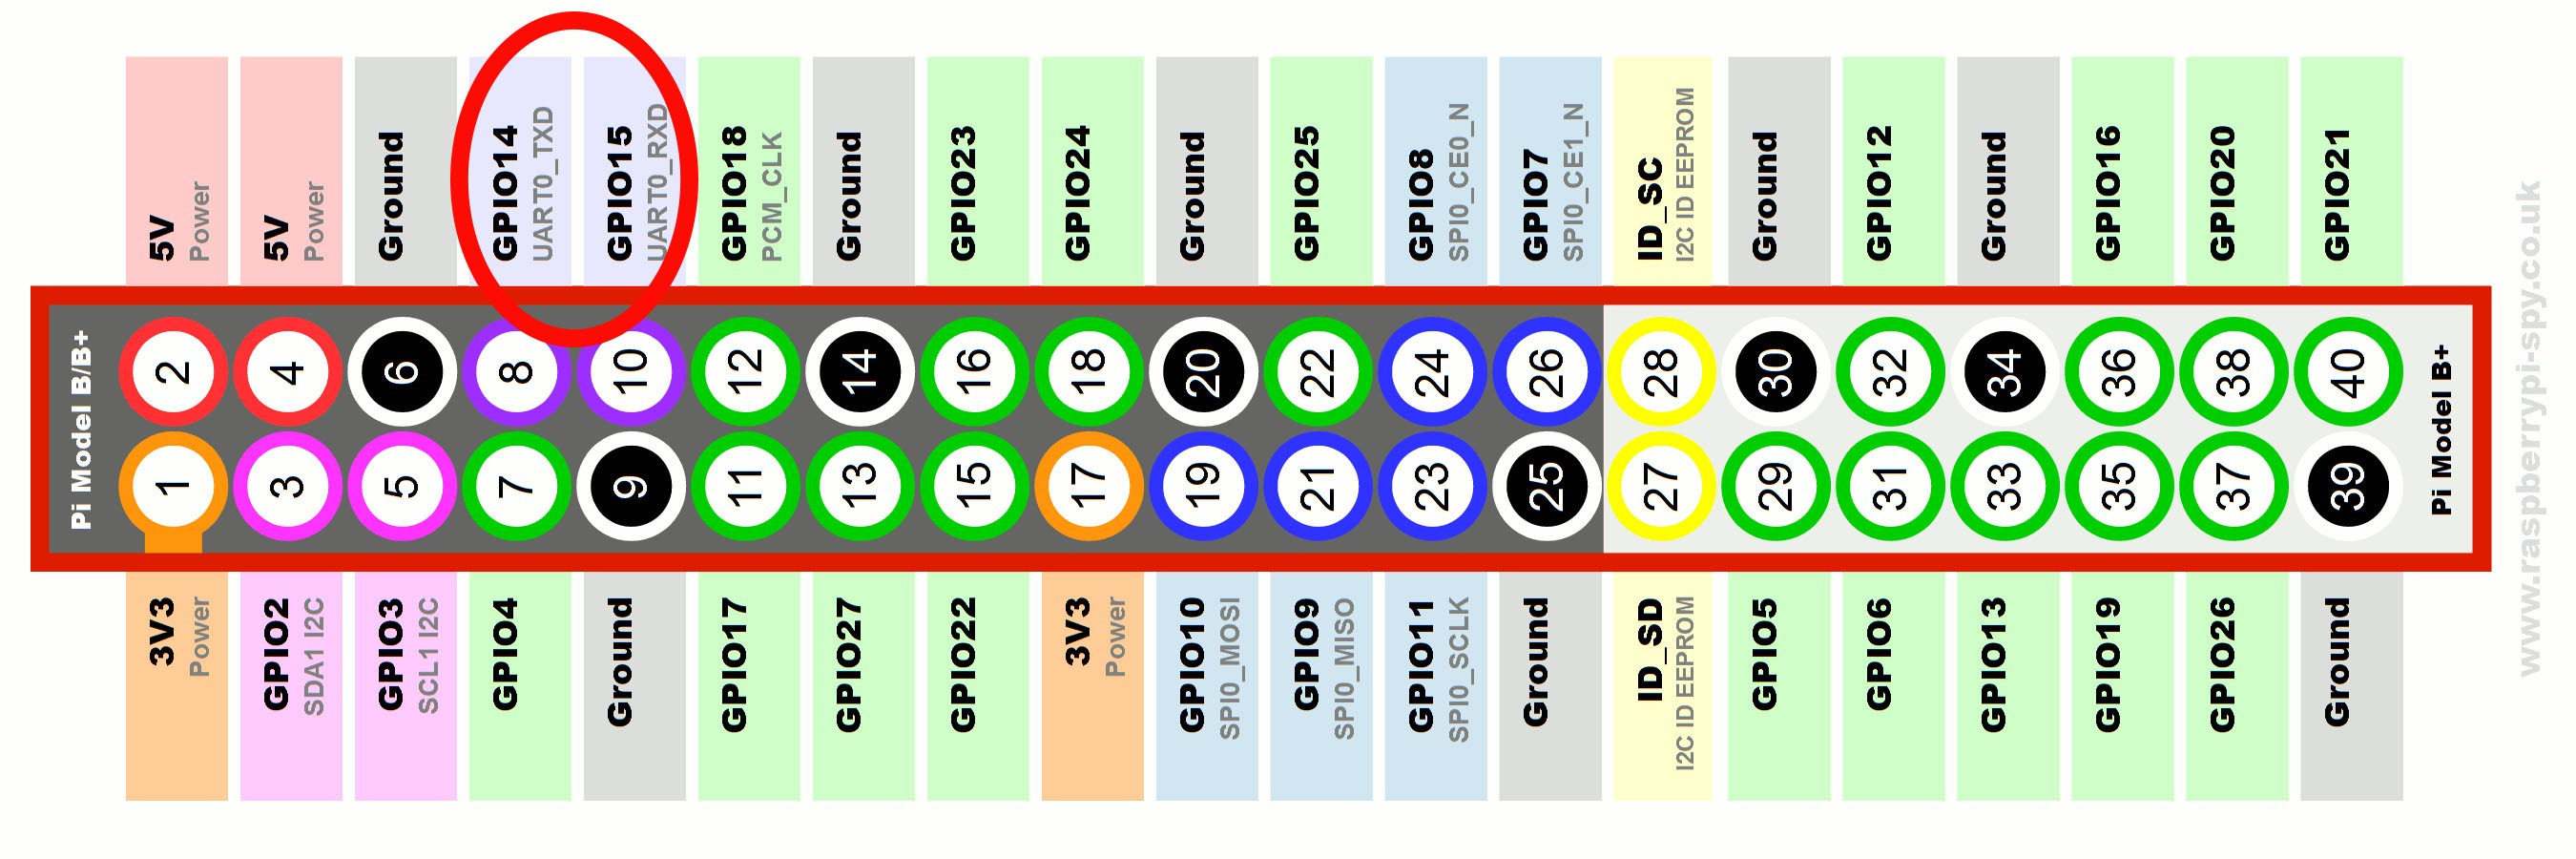
\includegraphics[scale=0.143]{images/tesi2.jpg}
 \caption[Raspberry Pi UART pins]{Highlight of UART reserved GPIOs}\label{fig:seconda}
 \end{figure}

\subsubsection{UART0}
The UART0 is a fully fledged asynchronous serial interface, abiding to the 
PL011 ARM specification \cite{pl011}. To properly run on real hardware, the
corresponding pins must be configured to use the alternate function number 0 with
no internal pull up or down.
Its register are located starting at the address {\tt 0x3F201000}, each of them
is 32 bits wide and they are organized as follows (some unimportant ones are omitted for brevity):
\begin{description}
    \item[Data:] this register contains the first character present in 
            the receive FIFO and can be written to send an outgoing character to 
            the transmit FIFO. Addidionally, it presents an error report of the ongoing
            connection, with a specific bit for every condition (overrun, break,
            parity, framing).
    \item[RSRECR:] a redundant register for error conditions.
    \item[Flag:] contains various flags on the current state of the UART, like 
            state (full or empty) of the transmit and receive FIFOs and whether
            the UART device is busy or idle.
    \item[IBRD:] integer part of the baudrate divisor: when configuring the device
            the baudrate is established as a floating point divisor prescaling
            the system clock. This is the integer part.
    \item[FBRD:] Floating point part of the baudrate divisor.
    \item[Line control:] this register manages configuration options like
            parity, number of stop bits, word length and FIFO abilitation.
    \item[Control:] this register controls the actual peripheral; mainly used
            for enabling and disabling the whole device.
    \item[IFLS:] interrupt FIFO level selection register. It is used to establish 
            at which percentage each FIFO (transmit or receive) triggers the
            corresponding interrupt. Possible values range from 1/8 to 7/8.
    \item[Interrupt mask:] allows to mask specific interrupts tied to the peripheral,
            such as those fired on reception and transmission of a character
    \item[Raw interrupt:] read only register updated with currently pending
            interrupts, regardless of the mask settings.
    \item[Masked interrupt:] same as the raw interrupt register but with the
            masked interrupt lines excluded.
    \item[Interrupt clear:] register to be written to clear pending interrupts.
\end{description}

Of all those registers, the only ones a student should really care about are
data, flag, interrupt mask, masked interrupt and interrupt clear. All the others 
are used for the initialization of the peripheral, which is handled by the 
hardware abstraction layer and should not be changed.

The serial interface is configured as 8 bit wide, no parity bit and with
a baudrate of 115200. The FIFOs are disabled for simplicity, so they act like 
a 1-character deep buffer.

\newpage

\subsubsection{UART1 or Mini UART}
The UART1 is part of the group of auxiliary peripherals, together with two SPI
interfaces. In comparison with UART0 it has much more restricted functionality,
but still enough for a simple educational project. For example, it does not 
provide framing error detection or parity bit management, features that are either
disabled or ignored even in its more complete counterpart.
To properly run on real hardware, the corresponding pins must be set to use the
alternate function number 5 with no internal pull up or down.
Its registers are located starting at the address {\tt 0x3F215040}, each of them is-32 bits
wide and they are organized as follows (some unimportant ones are omitted for brevity):

\begin{description}
    \item[IO:] reading from this register yields the first character present in the
            receive FIFO, while writing it inserts the data into the write FIFO.
    \item[IIR:] register for enabling receive and transmit interrupts. If the first
            bit is set an interrupt line is asserted whenever the transmission FIFO
            is empty; if the second bit is set an interrupt line is asserted whenever
            the reception FIFO is not empty.
    \item[IER:] register holding information about which interrupt is pending (if any).
    \item[LCR:] controls whether the Mini UART works in 8 bit or 7 bit mode.
    \item[LSR:] line control status; used to determine if the device is ready to 
            accept new data or if there are received characters to be read.
    \item[CNTL:] control register to enable (in a separate fashion if so desired)
            the receive and trasmit lines.
    \item[BAUD:] 16 bit baudrate counter, to be set directly to the desired value.
\end{description}
Again, since the abstraction layer takes care of the initialization procedure
the user should really care about four registers: IO, IIR, IER and LSR.
The serial configuration is the same as the UART0.

\newpage

\section{Interrupt Controller}
\label{gic}
The BCM2837 SoC has at least two devices acting as interrupt controllers. One of 
them is clearly defined in the peripheral datasheet \cite{bcm2835}, while the
other is not clearly identified but hinted at thorugh register definition in a later 
revision \cite{rev3.4}. Those are here arbitrarily named Base Interrupt Controller (BIC)
and Generic Interrupt Controller (GIC).
These two interrupt controllers are cascaded, meaning that 64 interrupt lines are 
wired to the BIC which in turn compresses them into 2 interrupt lines for the GIC
controller; additionally, the GIC also receives some interrupt lines from mailboxes
and USB.

 \begin{figure}[h]
 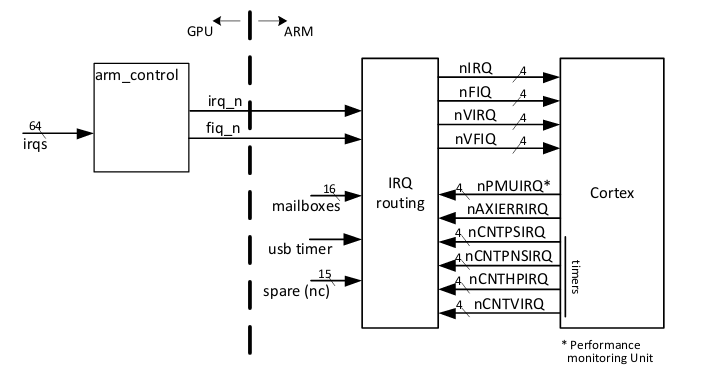
\includegraphics[scale=0.55]{images/tesi3.png}
 \caption[Interrupt Controllers]{BCM2837 interrupt controllers configuration}\label{fig:interrupt}
 \end{figure}
From a practical standpoint there are often several redundant registers indicating which interrupt
line is being asserted at any given moment. There is no apparent drawback in ignoring most
of them and just reading each device-specific register to discern which source fired
the exception, as the general interrupt organization is very confused and obscure. Interrupt functionality
was achieved mainly through examples and reverse engineering regarding the specific
device taken in consideration at the time.
What follows is a brief listing of interrupt related configuration for the devices
used in this work.

\begin{description}
    \item[UART] Both UART devices are cascated through the two interrupt controllers;
        although they can be checked via registers in both controllers, it is suggested
        to only read the Masked IRQ and IIR registers of the respective peripheral.
    \item[ARM timer] Being this an interrupt internal to the ARM processor its
        status has only been checked against the innermost interrupt controller (GIC).
        It is not clear whether it is present in the BIC as well.
    \item[Inter processor mailboxes] Possibly the sole source clearly
        depicted from the documentation, its presence can be understood from the 
        corresponding register in the Generic Interrupt Controller (as indicated
        by \ref{fig:interrupt}).
    \item[EMMC] Its interrupt lines are asserted by a device-specific register and
        seemingly nowhere else.
\end{description}

\subsection{Inter Processor Interrupt (IPI)}
In a multicore system such as the Raspberry Pi 3 the need arises for a privileged
communication channel between each core. The ARM Cortex-A53 does not provide an 
explicit method to do so, and it is left to the Generic Interrupt Controller to 
provide.
Similarly to the interface between ARM and Videocore there are mailboxes between
the four cores of the CPU as well.

The operation of those inter core mailboxes is much more straightforward than the
CPU-GPU counterpart. There are four mailboxes for each core and for each one the GIC
exposes three classes of control registers, for a total of 36 registers 
\footnote{Note: the first kind of register covers all four mailboxes for each core}.
\begin{description}
    \item[Mailbox Control] four registers of this type in total, one for each core
        and covering its four mailboxes. They enable an interrupt or fast interrupt
        line for each mailbox.
    \item[Mailbox Write-Set] four registers for each mailbox in every core, so 
        sixteen of them in total. They are write only and are used to put the
        actual data in the mailbox. Upon write the corresponding enabled exception
        (if any) is fired for the selected core.
    \item[Mailbox Read and Write-Clear] one register for each corresponding
        Write-Set register. They can be read to receive the data sent by writing
        in the Write-Set register, and have to be written to disarm the interrupt
        line. Each bit of the register is independent in firing the interrupt, so 
        to completely clear it the same content that was read from the register must
        be written back on it.
\end{description}

\clearpage{\pagestyle{empty}\cleardoublepage}
\chapter{Emulated peripherals}
\label{emulated}
The Raspberry Pi 3 (or any other version or model) does not have many peripheral
devices to toy with. In part this is due to its heritage of low resource board, 
and in part to extensibility through four generic USB ports and 40-pin header,
allowing for a wide range of HAT (Hardware Attached on Top) extensions and external
USB devices.
In the perspective of an educational project however this is a severe limitation.
While $\mu$MPS2 and $\mu$ARM can each bring five device types with eight possible
instances per type, the Raspberry Pi has only two really usable devices: the 
two serial interfaces (that strongly resemble $\mu$MPS2 terminals).

Other options cannot be considered for multiple reasons:
\begin{itemize}
    \item The screen is simple and usable, but lacks educational value. It is 
        nothing more than a buffer to write on; the GPU then manages actually
        sending the data to the screen.
    \item The EMMC interface is far too complex to be used by students. The professor
        would need either to spend a great deal of time and effort to explain how
        it works or provide a library to access it, in contrast with the philosophy
        of this work.
    \item The USB controller suffers a even worse degree of complexity, to the point
        where developing a support library would be a monumental task in itself.
        Last but not least, it is not supported by Qemu.
    \item The network interface is unfortunately not directly connected to the ARM
        but instead managed by the USB controller.
    \item Other auxiliary peripherals like the two SPI interfaces would be perfect
        for the task: although arguably too low level, many modern motherboards
        include SPI or I2C controlled peripherals, making it an intersting addition
        to the program. However, those are not supported by Qemu.
\end{itemize}

To mitigate this problem, three classes of new devices have been implemented as 
emulated peripherals in the hardware abstraction layer. Using $\mu$MPS2 as a reference,
these classes are tapes, disks and printers.

While building an entire emulator would give full control over the device interface,
in this work the emulation is carried on to the best level permitted by a bare
metal environment, leaking some imperfections on the exposed controls.

\section{Emulated Device Interface}
\label{emulatedinterface}
Initially emulated devices were made accessible via fake registers: simple pre-established
memory locations that were frequently polled (once every 100 $\mu$s) by the abstraction layer.
Though most similar to the $\mu$MPS2 approach, this idea had significant flaws.
\begin{itemize}
    \item fake registers had no read or write limitations; location that should
        logically have been read only could be modified without limit, leaving
        the device in an incoherent state.
    \item polling was a frail mechanism, prone to error and race conditions. 
         A real device starts working the moment
        its registers are written, while in this scenario the user had to wait 
        for the contents to be read by the abstraction layer. This leads to 
        an unintuitive programming path, requiring the user to either poll 
        for changes in turn or use an {\tt swi} assembly instruction to wait for
        the polling interrupt.
    \item generally speaking, it is good practice to avoid polling when possible.
\end{itemize}

A solution was found that strays from the previous work's approach but better
fits the new environment and allows for a cleaner emulation: using mailboxes.

Some of the peripherals on the BCM2837 board are already managed by the GPU
through mailboxes, like the HDMI controller or the on-board activity led. In 
a very similar way, the abstraction layer is notified of a new command for printers,
tapes or disks by a write to the inter core communication mailbox.
Specifically, the mailbox 0 of the first core is reserved for emulated devices control.
This behaviour is transparent to the user because it raises a FIQ instead of a 
normal interrupt, and thus it can be received at any moment.

A command to a emulated device is then issued by writing some value to the mailbox
0 write-set register of the first core, found at memory address {\tt 0x40000080}.
The value must have the following format: the two least significant bits are the
device number and the two following bits are the device class.
The upper 28 most significant bits should point to a 16-byte aligned address containing
a register structure for the selected device.

\begin{figure}[h]
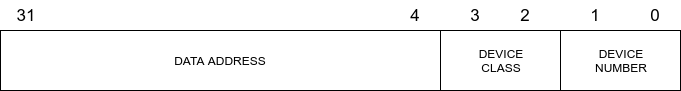
\includegraphics[scale=0.571]{images/tesi5.png}
\caption[Mailbox Structure]{Mailbox structure}\label{fig:mailbox}
\end{figure}

This should remind the reader of the mailbox communication protocol used by ARM
to talk with the Videocore, with the channel number encoded in the 4 least significant
bits. Since it is a mechanism already present in the system it fits naturally
in the development process.

The ``register'' structure that should be pointed by the mailbox address is nearly 
identical to the device register layout in $\mu$MPS2 and $\mu$ARM.

\begin{table}[h]
\begin{center}
    \begin{tabular}{|c|c|c|c|}
    \hline
    \rowcolor[HTML]{C0C0C0} 
    Field \# & Address   & Field name & Size    \\ \hline
    0        & base+0x0  & STATUS     & 32 bits \\ \hline
    1        & base+0x4  & COMMAND    & 32 bits \\ \hline
    2        & base+0x8  & DATA0      & 32 bits \\ \hline
    3        & base+0xC  & DATA1      & 32 bits \\ \hline
    4        & base+0x10 & MAILBOX    & 32 bits \\ \hline
    \end{tabular}
 \caption[Device Registers Layout]{Device registers layout}\label{tab:reg}
\end{center}
\end{table}

Every device can have special functions for each register; what follows is a
general description.
\begin{description}
    \item[STATUS] contains the device state.
    \item[COMMAND] contains the command code to be executed.
    \item[DATA0 \& DATA1] carry additional arguments for the command.
    \item[MAILBOX] is written by the system to notify the command has been carried on.
\end{description}

Since this structure is nothing but a user memory location, fields like \textbf{STATUS}
and \textbf{MAILBOX} are uninitialized at first; only \textbf{COMMAND}, \textbf{DATA0} and \textbf{DATA1}
must contain proper data. Once the abstraction layer has received the fast interrupt
and parsed the registers it copies the internal state of the device onto the
provided memory location, populating all of its fields.

After receiving the mailbox the abstraction layer sets the \textbf{MAILBOX} field
to 1. This however does not mean the operation has been finished successfully, because 
real world devices take time to operate; as such, there are fabricated delays between
commands and execution. Both the initial interrupt and the subsequent delay are 
handled at \textbf{EL1} by fast interrupts.

Once the execution is complete an interrupt is asserted. Interrupt lines for emulated
devices are emulated as well with a memory location allocated for the task, at 
base address {\tt 0x0007F020}.

\begin{table}[h]
\begin{center}
    \begin{tabular}{|c|c|c|c|}
    \hline
    \rowcolor[HTML]{C0C0C0} 
    Interrupt line \# & Address  & Device class & Size   \\ \hline
    0                 & base+0x0 & Timer        & 8 bits \\ \hline
    1                 & base+0x1 & Disk         & 8 bits \\ \hline
    2                 & base+0x2 & Tape         & 8 bits \\ \hline
    3                 & base+0x3 & Printer      & 8 bits \\ \hline
    \end{tabular}
 \caption[Emulated Interrupt Lines]{emulated interrupt lines.}\label{tab:reg}
\end{center}
\end{table}

Interrupt lines for emulated devices are nothing more than an array at a specific
memory address that is kept updated by the abstraction layer. Whenever an operation
terminates a bit is set for the user to clear; until that happens interrupts will
keep being raised in the form of a zero-delay timer (i.e. until there is an emulated
interrupt line asserted the abstraction layer sets a timer for 0 microseconds 
in the future, ensuring the kernel responsibility to clear it).\\

The next sections are dedicated to the specific device classes. The interface and
operating rules were copied almost identically from $\mu$MPS2, so the interested
reader is redirected to its documentation for the details \cite{pop}; here are listed
some general informations and implementation peculiarities.

In addition to the commands defined in $\mu$MPS2 there is another recurring instruction,
the \textbf{READ\_REGISTERS}, an alias for the value codified as {\tt 2}. This
command is instantaneous in every case and simply copies the device registers into
the structure specified in the mailbox. It substitutes reading the system registers
without causing any effect on the peripheral.

The next chapter covers in greater detail the inner mechanisms of the emulated 
devices.

\section{Printers}
MaldOS supports up to four parallel printer interfaces able to transmit a 
single byte of data at a time. Characters sent to a printer are displayed on 
the HDMI connected display in the printer's section.
The data structure expected by the abstraction layer is the same as every other
device (see table \ref{tab:reg}) despite the \textbf{DATA1} field not being used.\\
When the device writes receives a mailbox message and copies its state into the
register structure \textbf{STATUS} is updated with the current state of the device
(busy, ready, under error condition). Even an unrecognized or impossible command will
 result in this update, albeit followed by the proper error condition.\\
The \textbf{COMMAND} fields accepts directives to reset, acknowledge, print a
character or read the current registers. Commands issued while the peripheral
is busy will be ignored.\\
The printer's interface maximum throughput is 125 KB/sec.

\section{Disks}
MaldOS supports up to four readable and writable disk devices. The disk current
position is indexed by a combination of head, cilinder and sector to select
4KiB blocks of persistent storage memory.
Reading \textbf{DATA1} always returns the geometry of the installed disk: maximum
number of cylinders, heads and sectors.\\
When reading or writing a block the register structure should specify a pointer
to an adequately spaced memory range in \textbf{DATA0}. Disks are DMA operated, so the abstraction
layer will take care of moving requested information to or from the medium.\\
Whenever a command is issued the \textbf{COMMAND} field should be filled with
additional arguments, like the cylinder to reach or sector and head to read from.

The disk write and read speed are dependant on the (emulated) hardware and can 
be configured for each device before installing it.

\section{Tapes}
Tape devices are very similar to disks, with the two major differences being they
are read only and are accessed in a sequential fashion.
They are organized in 4KiB blocks as well, with each block terminating in a
4-bytes marker that is copied into \textbf{DATA1}. After a reset it reads 
\textit{TAPE START} and changes after reading a block or otherwise moving the
head. \\
Possible values for markers are \textit{END OF BLOCK}, \textit{END OF FILE}
and \textit{END OF TAPE}. They are used to navigate among the files that have
been assembled together when creating the tape.\\
Like disks they are DMA-operated and \textbf{DATA0} should contain a pointer 
to the memory block to populate.

\clearpage{\pagestyle{empty}\cleardoublepage}
\chapter{Project Internals}
In this chapter we describe in reasonable detail the source code of the 
project. The discussion will tipically hover at a structural level, depicting 
the design choices and code organization. This part will be most interesting for
those with the intent of maintaining or modifying the work, or to study ARM
bare metal development.

The size of the project is comparatively small, only reaching about 4000 lines of 
code. The real weight of this work does not lie in the actual software that was
written but in the idea and study of the environment, pioneering the possibility
of developing a proof-of-concept OS on real hardware instead of an emulator.

\section{Design Principles and Overall Structure}
Besides creating a convenient abstraction layer, the whole code base is written 
with the goal of being an understandable example of bare metal development. Particular 
care is taken in making sure that every function is readable and understandable
with a single glance even out of context and in using descriptive, self-explanatory
names. Where deemed necessary, comments help to further clarify what is happening.

Source files can be grouped in three main categories. First, the core of the abstraction
layer is comprised basically of the assembler entry point, the C entry point and
the interrupt handling routines. Second, a small library used internally to 
access hardware peripherals; logging routines, microSD card reading and writing, 
timer management. The third category contains the modules of the emulated devices like tapes and
printers, leaning on the previous utilities to create the illusion of physical
peripherals.

\subsection{Implementation Language}
The choice of language is severely limited by the bare environment and fell unsurprisingly
on C and Assembly. Such basic programming languages contribute to the overall simplicity,
as there are no particular patterns or constructs used beside raw memory management.

The Assembler compoment was kept to a minimum for ease of understanding; from
the moment the C stack is available there is no real reason not to jump into 
C code (unless the goal was to exercise Assembly programming, which is not our case).

Thus, there are only two Assembly source files: {\tt init.S} is the absolute first
entry point and provides initialization for system registers, interrupt vectors, 
bss section and multicore functionality; {\tt asmlib.S} contains utility functions
that make heavy use of general and specific purpose registers that would have
required inline Assembly instructions anyway if implemented in C.

\subsection{Build Tools}
Contrarily to the $\mu$MPS family of emulators, this work does not use the 
Autotool suite of building tools (GNU Automake and Autoconf) to manage source 
compilation and package installation.
Not having a newly created graphical interface there are no library dependencies
such as Qt, weakening the need for strict dependency check. 
This, together with a smaller overall codebase prompted the author to search 
for a simpler and more modern build tool, and the final choice is Scons.

Scons has the advantage of being much more flexible and easy to use when compared
to older tools. Instead of leaning on a brand new (and potentially cumbersome)
language to configure the build process it relies on an already existing one, well
received and praised for its approachable syntax: Python.

In fact, Scons can be assimilated to a Python library for declaring build dependency
trees. Its philosophy is similar to Make but brings a much cleaner syntax and 
user control over the process. 

\subsection{Linker Script}
The linker script is an essential piece when compiling for the Raspberry Pi 3. It has
to specify {\tt 0x80000} as the loading address for compatibility reasons with Qemu
and it ensures the initialization code is at the very beginning of the kernel image.
It also allocates some memory as stack to be used by the abstraction layer interrupt
routines.

\section{Initialization}
After loading all necessary components, the on-board GPU launches ARM execution at 
address {\tt 0x80000}. There, we can find the compiled code from the 
{\tt init.S} Assembly file.
The first operations are:
\begin{enumerate}
    \item Enabling access at \textbf{EL0} and \textbf{EL1} to the internal ARM 
        timer registers.
    \item Setting a separate stack for each core for internal interrupt handling.
    \item Enabling AArch64 execution state.
    \item Moving the execution level to \textbf{EL1} \footnote{The Raspberry Pi 3
     starts in \textbf{EL2}, while Qemu initially runs at \textbf{EL3}}.
    \item Setting up interrupt handling routines.
    \item Preparing execution for all cores: while the first core jumps to C code,
        the remaining ones are parked in a waiting loop, ready to be fired.
    \item The bss section (uninitialized data) is zeroed and the first core jumps
        to the {\tt bios\_main} function.
\end{enumerate}

From there control is passed to C, with another series of initialization routines:
\begin{enumerate}
    \item The memory locations dedicated to device emulation and user interrupts
        are cleared.
    \item Every real device is initialized: GPIOs, UARTs, EMMC, display.
    \item Every emulated device is initialized, building on the real hardware.
    \item Cores 1, 2 and 3 are unlocked from their parked state and set to 
        run an infinite wait loop.
    \item The user provided {\tt main} function is called.
\end{enumerate}

\section{Interrupt Management}
\label{regcorruption}
The core of the abstraction layer lies in the interrupt handling routines. We refer
to the handlers predefined in the abstraction layer as internal interrupt handlers;
 the students should define their own handlers, from now on referred to as user defined handlers.
There are 4 possible (and real) IRQ sources:
\begin{enumerate}
    \item ARM timer
    \item UART0
    \item UART1
    \item Mailboxes
\end{enumerate}
The {\tt main} function is assumed to never return; inside it the user should
prepare an appropriate time slice and then start executing the first process.
The time slice is set using the {\tt setTIMER()} function.
Note that {\tt setTIMER()} does not interacts with the ARM timer directly but 
through an internal delay system; since the physical ARM timer interrupt is also
used to ensure interrupts are fired on emulated interrupt lines sometimes a
0 $\mu$s delay is set. To avoid losing the user requested timer a simple array 
holds the next delay for every core and is restored when no more virtual 
lines are pending.

 Once the time slice is over the internal interrupt handler is called. 
 It checks for real or emulated pending interrupt lines and immediately
 passes control to the user defined interrupt handler.

 \begin{figure}[h]
    \begin{center}
 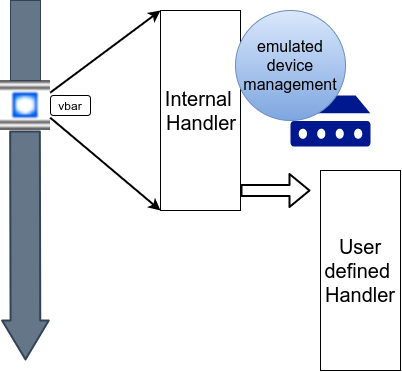
\includegraphics[scale=0.8]{images/tesi6.png}
 \caption[IRQ Switch]{Interrupt handling schematic}\label{fig:irq}
    \end{center}
 \end{figure}

 %TODO: fix everything

Other exception handlers, like the synchronous exception handler, are even 
simpler, reduced to passing control to the user defined routine if present.

The abstraction layer does mainly two things before passing control to the user:
\begin{enumerate}
    \item setting the stack pointer to a specified value for each core.
    \item setting \textbf{TTBR0} to the kernel page table, giving the illusion
        of different page tables for different exception levels, which simplifies
        significantly the whole virtual memory system.
\end{enumerate}
This meddling has a relatively negligible drawback: the interrupt routine is forced
to corrupt two general purpose registers.
 The conscribed registers are \textbf{X27}
and \textbf{X28}, and they should not be used for other purposes.

\section{Emulated Devices}
\label{emulateddev}
The idea behind emulated peripherals and their fabricated interface 
has already beed described in Chapter \ref{emulated}. Here we give a more detailed 
presentation about the principles under which they work.

A command to an emulated device is issued through a mailbox. For coherency reasons
interrupts are however disabled at execution level \textbf{EL1} (the execution
level of user defined interrupts). To maintain this precaution and still allow 
user code running at \textbf{EL1} to be properly served when sending a command, the
special mailbox used for emulated peripherals fires a fast interrupt request (FIQ)
instead.
Fast interrupts are kept obscured to the user and managed only internally (in fact,
for this single purpose). IRQs and FIQs are separated for historical reasons, so 
the abstraction layer can disable the former and enable the latter.

Some commands require a two-step management to more closely resemble a real peripheral.
The first step is the fast interrupt, and is present for every command. For longer
operations a virtual timer (different from the physical timer used through the
{\tt setTIMER()} function) is set to be executed by another FIQ interrupt after 
a certain amount of time.

\subsection{Tapes and Disks}
Tapes and Disks are very similar in their underlying functionality. While tapes 
are read-only and are accessed in a sequential fashion, disks can be written and
read at random. Their content is transferred as queried through a DMA system.\\
The tape can be viewed as a sequential list of 4KiB blocks, each block followed
by a marking 4 bytes delimiter denoting the nature of its content (last block of 
a file, last block of the tape or neither of those).
The disk on the other hand has blocks organized with a three dimensional indexing
that reproduces a head-cylinder-sector disposition.

When a command is issued to the disk or tape device a FIQ for the first core is immediately
fired. Depending on the command it might be evaded immediately or set a timer for
later to emulate hardware delay; commands such as \textbf{RESET} and \textbf{ACK}
finish on the spot, while operations like moving the device and reading/writing
 a block are postponed for a few milliseconds.\\

The actual content of both tapes and disks is saved as a file on the SD card. When the system 
boots it looks for files named {\tt TAPEn} and {\tt DISKn}(where \textit{n}
 is an index from 0 to 3) and considers them as installed. 
The file format for tapes and disks is identical to the one used by $\mu$MPS2: 
\begin{itemize}
    \item Tapes have a 4-bytes identifier right at the beginning, then 
        a list of 4 KiB blocks paired with yet another 4 bytes of ending marker.
    \item Disks have different identifiers at the start, then six 4-bytes configuration
        words describing the number of cylinders, heads and sectors plus the rotation
        speed, the seek speed and the data occupation ratio.
\end{itemize}
In fact, such files can be created and added to the microSD card using the same tool
distributed with $\mu$MPS2, {\tt umps2-mkdev}.

 \begin{figure}[t]
    \begin{center}
 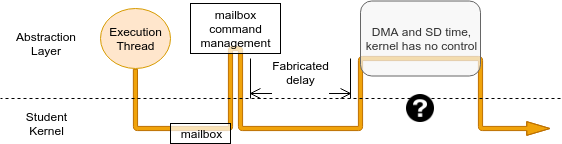
\includegraphics[scale=0.65]{images/tesi13.png}
 \caption[HAL Execution Thread]{The user provided kernel might realize there are some
 ``gray zones'' in its execution time when the SD card is accessed. Proportions
 in the figure are exaggerated.}
 \label{fig:executionthread}
    \end{center}
 \end{figure}

Thanks to the mailbox interface the illusion of a real hardware peripheral receiving
orders and reporting with interrupts is almost perfect. The only real discrepancy
is the Direct Memory Access function: from the student's perspective the device
is writing or reading to or from the specified address; a scrupulous observer
however may notice how the memory transfer operation is carried on instantaneously,
and that there are comparatively big time gaps in kernel control when it happens,
as depicted in figure \ref{fig:executionthread}.
This is because the emulation layer takes place on the same execution thread of
the kernel, forcing to share time and resources when the command is carried on.

Overall, this should not be a major concern for a novice approaching OS development.

\subsection{Printers}
Printer devices are little more than an adaptation of the HDMI display port.
The Videocore IV manages almost everything: it holds a block of memory designated
as framebuffer to display on screen in its own memory space and allows the ARM
CPU to modify it freely. A binary font is included in the {\tt .elf} file to 
print textual information and the screen is divided in four sections for different
printer instances.

Printing a character merely writes it on screen, left to right and top to bottom.
This is somewhat different from $\mu$MPS2, where printers more faithfully output
their results to text files. To the author this approach seemed a little confusing,
because it is not possible to view the output in real time and since other media
devices are just files on the host filesystem they often felt like simplified 
tapes. Moreover, having them on the microSD filesystem would increase the need
for a more immediate access since the latter needs to be mounted before reading
the output file.

It would be indeed possible to flush printers on {\tt PRINTERn} files just like
tapes and disks, but doing so would significantly complicate the small FAT32 
library included in the project. Disk and tapes are arbitrarily big but have a
statically allocated size: printers need to grow indefinitely, demanding a function
to allocate more blocks on the file system.

\subsection{Timer Queue}
The second step of some device commands is scheduled for execution after a while;
since there is only one virtual timer at \textbf{EL1} to fire scheduled interrupts, this would
eventually overwrite other pending timers. The physical timer is already allocated
to schedule time slices, and two interrupts would not be enough anyway.
To prevent this MaldOS uses a set of queue managing functions to 
schedule multiple virtual timers at once. 
The ROM function {\tt setTIMER()} does not interact with the queue, but uses
the physical timers instead.\\
The queue is kept ordered from the first timer that will occur to the last.
When an interrupt is fired all the timers that were scheduled before the
current time are popped out of the queue, and the first remaining element (if any)
is scheduled again.

When a virtual timer for an emulated device is served it is likely that the
corresponding interrupt line will be asserted following command completion. 
For this purpose a phony ``0 microseconds'' \textbf{physical} timer is scheduled to 
ensure that the line is serviced as soon as the FIQ terminates.

Interestingly, the implementation of this module is heavily inspired by the list
managing routines found in a past solution to phase 1 of the KayaOS project, 
covering process and semaphore queues.

\section{Hardware Library}
Modules under the {\tt source/hal/} subdirectory contain functions to conveniently access 
and use hardware peripherals. They serve a purpose mainly for usage internal to 
the project, as the abstraction layer does not normally expose those functions
(e.g. reading and writing the microSD card to emulate disk and tape devices).
They could however be seen as one of the many educational examples about 
bare metal programming for the BCM2837 and ARM processors in general.

Notably, since disk and tape devices are ``plugged'' into MaldOS as files onto
the microSD, a small FAT32 file system library was necessary over the EMMC controller
integration.
The system expects a master boot record signaling a first FAT32 partition. There
root entries (directory navigation is not supported) are listed and searched for
the necessary \textit{DISKn} and \textit{TAPEn} files. Since both those device
classes have a fixed size the library does not support file growth or shrinking,
only read and write with eventual modifications.
Partitions of any size permitted by FAT32 are accepted: the file allocation table
is only partially loaded in main memory as a cache of cluster pointers.

\section{Memory Management Unit}
\label{halmmu}
Using the MMU can be considered a higher level of complexity in its own right.
One of the improvements brought by $\mu$MPS2 over $\mu$MPS was the possibility 
of having it disabled for the first phases of the project, since the real 
MIPSEL architecture had the virtuam memory translation constantly active.
In truth, there is little reason in practice to turn off such a feature: a microprocessor
is born to run an Operating System, and every Operating System worthy of its name
virtualizes memory for its processes. A smoother learning curve is quickly 
sacrified for the sake of efficiency.\\
Possibily because ARM lives in a world closer to embedded, low power, low resources,
time constrained applications, its MMU devices are usually activated on demand,
which is why the first phases of Kaya are still possible on the Raspberry Pi 
without having to worry about page tables.
When activated, however, the MMU leaves little to no room for anything else: it 
expects, from the very beginning of execution,
 the kernel to be loaded starting from a special address to use a separate
page table from normal processes. This proved hard to integrate with an abstraction
layer that provides a great deal of initialization code without knowing whether
virtual memory will be used.

The solution is to move only the entry points of the user kernel, which are
two: the interrupt address found in the \textbf{VBAR} register and the first
{\tt LDST()} function call to launch the first user process. 
On the interrupt table side the \textbf{initMMU()} function
initializes system registers, disabling every cache and setting up for full
range, 4KiB blocks page tables (using a simple identical mapping for the first
translation function) and moves \textbf{VBAR} over to {\tt 0xFFFF000000000000},
making sure that \textbf{TTBR1} is used when jumping to the kernel. If the handler
is reached through that jump for all intents and purposes the kernel believes to 
be running at the far end of the main memory.
As for the first process context switch, it is a tricky situation: after enabling
the MMU but before loading the process state the kernel is still using \textbf{TTBR0}
because its entry point did not pass through the ``rigged'' \textbf{VBAR} register;
therefore the TLB cache will contain entries from the kernel page table.
The very last instruction before using {\tt eret} to switch to \textbf{EL0} loads
the new \textbf{TTBR0}. Even so, the {\tt eret} instruction will fetch the
new, user level page entry while still running as the kernel and
 cause an instruction abort for security reasons.
To avoid this, one must make sure to call {\tt LDST()} through \textbf{TTBR1},
which can be achieved by jumping to the address of {\tt LDST} plus the most significant
two bytes of the 64-bits register. In this way the kernel tables will be used 
until the user process is actually running.\\
Note that this problem should not present itself if the process' code is loaded
in a different memory block. Nevertheless it is a theoretical inconsistency and
should be considered.

The only other alternative would be to pretend to load the entire binary at that
address by specifying it in the linker script, and then setting up the MMU at 
boot, before even jumping to C code. For reasons already listed, this was not
acceptable.

\subsection{Design Choices}
While constructing the virtual memory environment the author came across design 
crossroads where the decision was not driven by technical considerations, but
rather educational ones.
For example, the abstraction layer can let students avoid ASID management by 
simply flushing the TLB cache every time there is a context switch; if not,
failure to setup proper process IDs will result in abort exceptions. Ultimately 
the latter approach was taken, leaving to the user to write a new ASID to 
\textbf{TTBR0} every time a new process is launched.
Again, user-defined handlers are written to special memory locations as addresses
to jump to; if the MMU is active said addresses must be changed in order to 
have the CPU refer to \textbf{TTBR1} instead of \textbf{TTBR0} when calling those
functions. This nuisance can be handled automatically by the abstraction layer
(and indeed it is in the final implementation), but one could instruct students
to change the handler's address after enabling the MMU.

Those choices are subjective and could be easily changed.

\section{Exception Levels and Virtualization}
The ARMv8 specifications counts a great deal of features for virtualization
purposes. One of the four exception levels, \textbf{EL2}, is defined as the
hypervisor level and has responsibilities revolving around multiple guest OS management,
abstraction of system registers, nested virtualization of page tables (virtualized
virtual memory, so to speak) and device emulation. Some functions at \textbf{EL3} 
are connected to those concepts, but it is a level mainly focused on TrustZone 
technology and security. \\
Many of the ideas enumerated in this description are at the base of this project,
so one would naturally expect said features to be exploited to some extent.
Although the possibility is not ruled out by the author, up until the time of 
writing the route of \textbf{EL2} has been deemed unattractive for the development
of MaldOS.

After a thorough analysis, this should not come as a surprise. The hypervisor 
component that ARM refers to is for a complete Operating System to be taken advantage
of in the context of multiple virtual guest OS hosting; while intuitively an 
abstraction layer emulating multiple device classes and a simpler develoment 
environment has many common points, it is also significantly different. Therefore,
many configuration options offered by the hypervisor that could bring improvements to this
work ultimately fail to fit into it. The following sections portray the most 
notable ones.

\subsubsection{Trap General Exceptions}
\textbf{EL2} configuration is controlled by \textbf{HCR\_EL2}, a 64-bits 
long register with many choices in the matter of virtualization. The number
of available fields actually vary depending on the implemeted version of the
specification: the last ARMv8.3 uses 44 bits, but the Cortex A-53 processor was
created when version 8.0 was being defined, thus having only 33 usable bits.
Out of those fields the most prominent one is \textbf{TGE}, short for Trap General
Exceptions. When the \textbf{TGE} bit is set all exceptions that would normally
be executed at \textbf{EL1} are routed to \textbf{EL2} instead.\\
This option has the potential to greatly simplify the actuation of an abstraction
layer. Executing at the same level of the assisted code weakens it, forcing some
tradeoffs with emulation fidelity: for example, having two separate exception
levels could mean that the abstraction layer never needs to worry about virtual
memory as MMU settings are banked between levels, avoiding the register 
juggling uncovered in section \ref{halmmu}.
Unfortunately this result is not achievable, as an active \textbf{TGE} apparently
 means \textbf{EL1} is not accessible altogether. {\tt eret} instructions that
 would lower the exception level to 1 are treated as illegal exception returns 
 and maintain \textbf{EL2} privilege instead (carrying on execution from where
 the return should have started). If the abstraction layer is unable to 
 return to \textbf{EL1} when leaving the user code in control there is no point
 in working at \textbf{EL2} in the first place.\\
 Considering this behaviour it is unclear what purpose the \textbf{TGE} bit
 is supposed to serve, especially since another field (\textbf{E2H}) seems to 
 lead to the exact same scenario where the host Operating System lives in \textbf{EL2}
 instead of \textbf{EL1} \footnote{It should be noted that the \textbf{E2H} is 
 only available from version 8.1 of the specification.}.

\subsubsection{AArch32}
Section \ref{raspberry3} hints at the 32-bits compatibility interface of ARMv8, 
an essential property of all 64-bits architectures to allow execution of legacy
software. The \textbf{RW} bit of the \textbf{HCR\_EL2} register controls the
execution state of lower exception levels. In the scope of an educational project
the 32-bits architecture could be seen as more historically interesting and
appropriate as a first approach to the field; for this work however more value
was given to clean structure and modern perspective, and AArch64 was chosen.

\subsubsection{Trap System Registers Accesses}
Among the different variations that \textbf{HCR\_EL2} allows for there is the 
option to trap several memory accesses, both read and write, or certain instructions
(like TLB maintainance) to \textbf{EL2} with the intent of hijacking the result.
This possibility was not found to be useful in the context of this work.

\subsubsection{Partial Exception Routing and Virtual Exceptions}
In opposition to the \textbf{TGE} complete superseding of \textbf{EL1} by
\textbf{EL2} there are also separate fields in \textbf{HCR\_EL2} that allow
for single exception classes to be routed to a different level (\textbf{AMO}, 
\textbf{IMO}, \textbf{FMO} fields, corresponding to serrors, interrupts and
fast interrupts respectively).\\
Those fields share some of the advantages listed about general exceptions routing
while still retaining the possibility to return at \textbf{EL1}.
Moreover, when the corresponding routing bit is enabled another field permits the
hypervisor to set a virtual exception that lower levels will see pending and that
could be used to more properly emulate $\mu$MPS2 devices.\\

This situation is not perfect either. First, not all interrupt classes are subject
to this configuration, leaving out synchronous exceptions caused by instructions
like {\tt SVC}, used by system calls. While it is still possible to implement
the {\tt SYSCALL()} function as an {\tt HVC} call, the difference in exception
management is somewhat disorienting.
As for virtual interrupts, they still have to be taken and handled directly by 
\textbf{EL1}. By committing to this choice the abstraction layer would find itself in an 
uncomfortable position with overhead handlers for both \textbf{EL1} and \textbf{EL2}
instead of routing everything to \textbf{EL2} and then gracefully returning to 
\textbf{EL1} for user-defined routines, adding the complexity of the hypervisor
without solving completely \textbf{EL1} related problems (i.e. MMU register 
switching).

Overall, these options seem to be tailored around different objectives, so they
all fail to fix this project's main flaws or make other problems emerge.


\clearpage{\pagestyle{empty}\cleardoublepage}
\chapter{Student's Perspective}
This chapter describes what MaldOS exposes to a student to develop a toy OS:
provided ROM functions and mapped memory addresses that were decided and defined
taking inspiration from Kaya and $\mu$MPS2.
Barring some minor details, the illusion of touching an ARM system directly should
be perfect for a novice. That being said, ``jailbreaking'' out of MaldOS is 
fairly easy; the abstraction layer relies on a good willed user to be used at 
most efficiency.\\
As a first, general rule, direct interaction with system registers is
unnecessary (if not implicitly forbidden). Students can use a series of functions
exposed by the abstraction layer to perform configuration and management.

\section{ROM Functions}
Strictly speaking, there is no Read Only Memory on the BCM2837. This section is 
dubbed ``ROM Functions'' in reference to the precompiled routines provided as 
object files by $\mu$UMPS2 and similar emulators.
Those functions include:
\begin{description}
    \item[HALT()]: terminates the calling core execution, stopping in an endless loop.
    \item[PANIC()]: similar to \textbf{HALT()}, prints a kernel panic message before
        stopping.
    \item[WAIT()]: pauses execution until an interrupt occurs. Normally this is 
        achieved by the {\tt wfi} Assembly instruction; under MaldOS however multiple
        interrupts (FIQ) are fired without the user knowing, so the single instruction
        would be unreliable. The \textbf{WAIT()} function works because it checks
        on a spinlock opened by the abstraction layer when a real interrupt is 
        reached.
    \item[LDST(void *addr)]: Load State function call. Reads the address to load
        a system state: general purpose and system registers to resume execution
        of a saved process. Used by the kernel to context switch to a process.
    \item[STST(void *addr)]: Store State function call. Writes the current execution
        state to the specified address; used by the kernel to save the interrupted
        process and resume it later. The saved state format is a structure (see
         \ref{lst:state}).
    \item[getCORE()]: returns the id of the core currently executing the function.
        Its implementation simply reads the \textbf{MPIDR} register.
    \item[getTOD()]: get Time of Day function. Returns the number of microseconds
        elapsed since reset, reading it from the internal ARM
        timer registers. Since the architecture is 64 bit, the returned value 
        is a complete 64 bit {\tt unsigned long}, as opposed to the split 
        \textbf{getTODLO()} and \textbf{getTODHI()} found in $\mu$MPS2's ROM.
    \item[setTIMER(unsigned long us)]: a routine to set the next timer interrupt to 
        be fired {\tt us} microseconds in the future.
    \item[initMMU(unsigned long *table)]: function to initialize the memory 
        management unit. Its argument is the initial page table to set to both
        \textbf{TTBR0} and \textbf{TTBR1}; the kernel page table, so to speak.
    \item[isMMUACTIVE()]: function returning either 1 or 0, depending whether
        the MMU for the current core has been activated or not.
    \item[SYSCALL(unsigned int, unsigned int, unsigned int, unsigned int)]:
    function used to invoke a system call interrupt. In truth, nothing more than
    the {\tt svc \#0} Assembler directive.
\end{description}

These functions are linked in the {\tt .elf} of the abstraction layer, thus can
be simply referenced in the code after proper inclusion. When compiling separately a
standalone executable to be loaded in RAM for the most advanced phases of Kaya
this is not contemplated, as it would link the whole HAL to every binary.
In this case it is left to the student to implement ROM functions: in reality, only
\textbf{SYSCALL} is needed for a normal process, and it has a one line implementation.
\newpage
\begin{lstlisting}[label={lst:state},caption={Process state format},language=C]
typedef struct _state_t {
    uint64_t general_purpose_registers[29];
    uint64_t frame_pointer;
    uint64_t link_register;
    uint64_t stack_pointer;
    uint64_t exception_link_register;
    uint64_t TTBR0;
    uint32_t status_register;
} state_t;
\end{lstlisting}

\section{System Initialization}
The student's kernel entry point is the {\tt main} function. The first task of 
the Operating System should be populating the custom interrupt routines: contrarily 
to $\mu$MPS2 interrupt handlers are not specified with a full process state, but
condensed into just the function and the stack pointer. The function pointer must
be loaded into the {\tt \_HANDLER} locations, while the stack pointer is higher 
up and there is one for each core. There are no separate stack pointer for different
exceptions: if an exception is fired from the kernel handler, the stack pointer
is kept the same.
An example of initialization sequence could be
\begin{lstlisting}[language=C]
*((uint64_t *)INTERRUPT_HANDLER)   = (uint64_t)&interrupt;
*((uint64_t *)SYNCHRONOUS_HANDLER) = (uint64_t)&synchronous;
*((uint64_t *)KERNEL_CORE0_SP)     = (uint64_t)0x1000000;
*((uint64_t *)KERNEL_CORE1_SP)     = (uint64_t)0x1002000;
*((uint64_t *)KERNEL_CORE2_SP)     = (uint64_t)0x1004000;
*((uint64_t *)KERNEL_CORE3_SP)     = (uint64_t)0x1006000;
\end{lstlisting}

After this, the first process should be created and loaded with a proper time
slice set as timer interrupt. The memory address from where processes can use 
stack starts where the kernel ends; said value is provided for convenience by 
the {\tt \_kernel\_memory\_end}, defined in the linker script.

 \begin{figure}[h]
    \begin{center}
 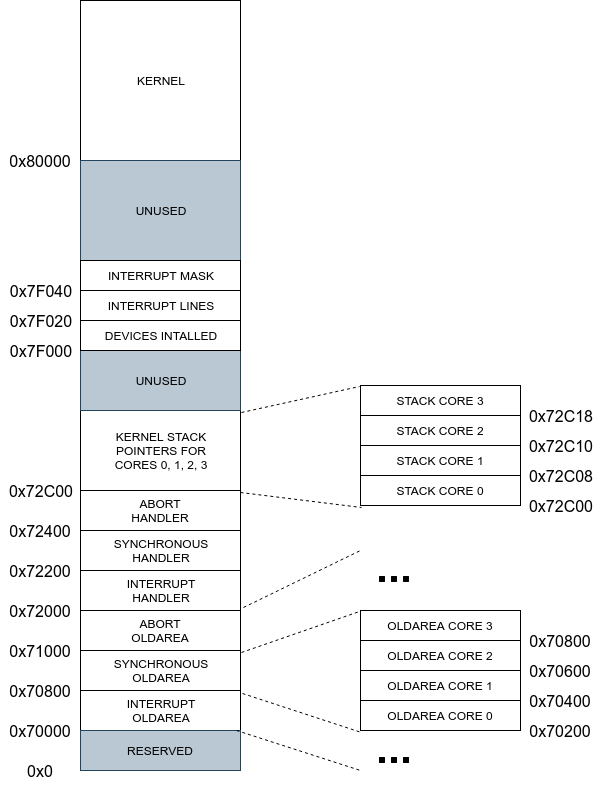
\includegraphics[scale=0.55]{images/tesi14.png}
 \caption[Memory Map]{Memory locations for interrupt old areas, handlers 
 and stack pointers}\label{fig:memmap}
    \end{center}
 \end{figure}

 \newpage

\section{Exceptions}
By default, exceptions are handled at \textbf{EL1}. Control is given to the 
specified handler with normal interrupts disabled but fast IRQs enabled; the user
is not supposed to change this settings, and doing so might result in untested
behaviour.
Thus, nested interrupts are not present. Interrupt exceptions are fired
for the student's kernel if a physical device requires it (UART) or if an 
emulated device is asserting its line; while an interrupt line (real or 
emulated) is pending and not masked, the interrupt handler will be called repeatedly
until it is properly acknowledged.
Since interrupt lines for emulated devices are nothing more than RAM locations
it is possible to forcibly deassert them by simply writing 0 instead of using
the provided \textbf{ACK} command. This should not be done and can lead to 
unpredictable outcomes.

Synchronous exceptions (namely, system calls) are very simple; on {\tt SVC} 
instruction the provided handler is called, and parameters can be passed using
general purpose registers. In fact, to properly return a value from a system call
the state saved in the corresponding \textit{old area} must be loaded with a modified 
{\tt X0} register.\\

Abort exceptions work similarly. Note however that unlike $\mu$MPS2, where TLB
faults were part of the normal workflow, MaldOS does not contemplate recoverable
aborts. The abort handler is however generic, and the possibility is not ruled
out.

Whenever an exception is fired, the handler is loaded using the specified stack
pointer for \textbf{EL1} and the executing core; if an exception condition happens
while at \textbf{EL1} (e.g. an abort or a system call, even if it does not make 
sense to invoke one when at kernel level) the stack pointer is kept the same
and grows from where it was left.

\section{Multicore}
MaldOS approach to multicore functionality is very simple. Exception handlers 
are shared among all cores, leaving to the user the responsibility to separate
routines based on the executing actor. Old areas where states are saved and stack
pointers on the other hand are defined in a per-core basis. Every core can have
its exceptions and handle them accordingly.

After reset and initialization cores 1, 2 and 3 are left stuck in a wait loop and
should be moved from there using core mailboxes to trigger interrupt handlers.
Inter Processor Interrupts (IPI) are completely transparent and work as defined
by the ARMv8 specification. The only exception is the first mailbox of the first
core, reserved for emulated peripheral management. Data written to this mailbox
is interpreted as a pointer to a device registers-holding structure and is not
controlled by the student provided kernel.
Other mailboxes on the other hand will immediately cause an interrupt in the
corresponding core. Mailbox interrupts must be cleared by writing the same data
in the write-clear register.

\section{Devices}
The student can use two classes of devices on MaldOS: emulated or real peripherals.

\subsection{Real Peripherals}
The only real peripherals accessible from the abstraction layer are the two 
built in serial interfaces, UART0 and UART1.
Section \ref{serial} describes in greater detail the register configuration for
said devices. Although clearly more complex and convoluted when compared to the
clean interface for $\mu$MPS2 emulated devices, it is believed the handful of 
registers needed to use UART1 and UART0 is still well within reach for a computer
science undergraduate student. Similarly to flying a plane, the hardest
part is taking off, and device initialization is already prepared by the abstraction
layer when the user kernel gains control.\\
Interrupt handling is self contained in specific device registers; once enabled
the exception routine will behave as expected, continously being called until 
the specific acknowledgement is delivered.

\subsection{Emulated Peripherals}
The emulated peripherals interface is kept almost identical to the $\mu$MPS2 
approach, and is detailed in sections \ref{emulated} and \ref{emulateddev}.
As mentioned before the commands are passed to the emulation layer with a memory
structure shared through the first core's first mailbox (unavailable for other
purposes). The memory address must be 16-bytes aligned, as the 4 least significant
bits are used to index the device the command is meant for.

\section{Memory Management Unit}
The MMU operation is described in depth in chapter \ref{mmu}. It is a complex 
device, unsuitable for undergradates. This complexity is, in the author's opinion,
very much intrinsic in the nature of virtual memory management, and little can
be done to ease it; even if possible it would not make sense to further simplify it as 
it would lose most of its educational value.
Therefore, the MMU interface has been left mostly untouched by the abstraction layer.\\
The sole real interference is copying \textbf{TTBR1} into \textbf{TTBR0} when 
handling an exception to make sure the memory can be accessed without trouble 
even at \textbf{EL1}. If this was not the case the kernel could end up receiving 
entry results of the process that was paused.\\
This passage is made essential by the fact that the MMU should be easily turned
on and off without changing too much of the original code. Real OSes like
Linux simply enable virtual addresses from the beginning and load the kernel
code at the far end of memory, where \textbf{TTBR1} is referenced for page tables.
Moreover, Qemu does not allow for loading addresses other than the default 
{\tt 0x80000}. \\

Other than that, the MMU is entirely managed by the user, even if
registers should not be directly accessed and instead modified only through 
{\tt initMMU()} and {\tt isMMUACTIVE()} ROM functions.
Just like $\mu$MPS2, how far one should go into implementing virtual 
memory policies is up to the professor or course using this tool. For
example:
\begin{itemize}
    \item Page tables support a Dirty Bit Modifier field; when an entry is found
        (either in the TLB cache or after a table walk) that has the DBM bit 
        cleared an MMU fault is raised expecting the software to handle the
        situation and re-try the same memory request. This is usually used 
        to only load memory blocks in memory when they are accessed, thus
        allocating less physical memory for each process.
    \item To avoid confusion where multiple processes find the same cached entries
        in the TLB each one of them should be paired with an ASID copied to the
        \textbf{TTBR0} register. If page entries are then marked as non-global
        using the \textit{nG} bit a TLB search hits only if the current ASID is equal
        to the one saved with the entry.
    \item In an exaggerated simplification the TLB cache can be flushed every time
        a context switch occurs. In this situation no ASID is needed as the stale
        entries are just wiped before they can cause issues.
\end{itemize}

Note that the memory management unit configuration is set on a per-core basis:
there can be cores where virtual memory is enabled and active, and others where
normal physical memory is used.


\clearpage{\pagestyle{empty}\cleardoublepage}
\chapter{Usage and Debugging}
\section{Final Result}
The final result of this work consists, from the user perspective, solely of 
two files: {\tt hal.elf} and {\tt hal.ld}.
The first is the the hardware abstraction layer compiled for an ARM64 target, 
containing system initialization and emulated devices management; the second is 
its linker script, to be used to link an application to the hal.

The hal performs all the necessary routines and then calls a {\tt main} function.
There is a weak-defined {\tt main} included with the hal that just echoes every
character received on UART0 that is supposed to be overwritten by a new {\tt main}.
symbol.
From there, the user provided code is expected to write specific memory addresses
to define new exception handlers and control emulated devices. 

One of the objectives of this work was to avoid creating ad hoc software and
relying as much as possible on widespread tools. Because of this, there is no
custom package like the $\mu$MPS2 emulator to install; instead the user needs
a proper cross compile toolchain for ARM64 (or an ARM64 device, like the Raspberry
Pi itself) and eventually Qemu.

\section{Compiling}
\label{compiling}
MaldOS provides a single {\tt .elf} file containing initialization code, abstraction
layer and some functions; given that, there are several ways to compile it 
into a project. Here an example is shown, where a single module contaning the {\tt main}
function is linked to the HAL.

\begin{lstlisting}[language=bash]
$ aarch64-linux-gnu-gcc -o main.o -c -Wall -ffreestanding \\
    -nostdlib -nostartfiles -O0 -g -march=armv8-a \\
    -mtune=cortex-a53 -fPIE -ffixed-x27 -ffixed-x28 \\
    -Iinclude/app main.c
$ aarch64-linux-gnu-ld -o app.elf -r main.o$
\end{lstlisting}

Each command option has its own meaning:
\begin{description}
    \item[-Wall] requires to print all warnings during compilation. Not Strictly
        necessary, but good practice.
    \item[-ffreestanding] assert that compilation targets a freestanding 
        environment, one in which the standard library may not exist and program 
        startup may not necessarily be at main.
    \item[-nostdlib] instructs not to use the standard system startup files or 
        libraries when linking.
    \item[-nostartfiles] commands not to use the standard system startup 
        files when linking.
    \item[-O0] is the optimization level; here it is 0, with no optimization at all.
        One might specify other levels, but in a project where the focus is on 
        the learning experience and not in performance compiler meddling should 
        be kept to a minimum.
    \item[-g] includes debugging symbols into the executable.
    \item[-march=aromv8-a] specifies the target architecture.
    \item[-mtune=cortex-a53] specifies the target processor.
    \item[-fPIE] generates position independent code; it is necessary for when
        the executable will be linked with the abstraction layer in the next step.
    \item[-ffixed-x27 -ffixed-x28] instucts the Assembler generator to avoid using
        general purpose registers \textbf{X27} and \textbf{X28}. 
        As described in section \ref{regcorruption}
        those are corrupted during context switch, and thus are not available.
\end{description}

Unless otherwise specified, all options are strictly necessary for a working 
result. The absence of some flags might not create immediate issues but are 
nevertheless to be considered a mistake (e.g. registers \textbf{X27} and \textbf{X28}
are rarely used).

Given a compiled elf with the user's code called {\tt app.elf} and assuming to
use {\tt aarch64-elf-gcc} as a cross compiler, the process to create a kernel image
would be 
\begin{lstlisting}
aarch64-elf-ld -nostdlib -nostartfiles -Thal.ld \
    -ooutput.elf hal.elf app.elf                                                                                                                                    
aarch64-elf-objcopy output.elf -O binary kernel8.img
\end{lstlisting}
The resulting binary can then be placed on a microSD card and run on a Raspberry Pi 3
or on Qemu.

\section{Qemu}
\label{qemu}
Since version 2.12 Qemu supports a Raspberry Pi 3 emulated machine.
The official version for the Linux distro of choice may be less recent, in 
which case the user needs to compile the package from source.
 Particular care was taken in assuring the same code runs with no discernible difference on
the emulator and the device, which was not a difficult task.
Usually, in the rare situations where virtual and real boards differ in their
behaviour the real hardware is in the right (as one would expect).
Some examples found along the way are:
\begin{itemize}
    \item Uninitialized memory location will inevitably contain null values if 
        running under Qemu; the real world RAM is not so clement, and will live 
        up to the tale of having its content randomized after a reset.
    \item The MMU memory configuration includes distinguishing between device
        and normal memory: while the latter ban be subject to caching to increase performance,
        the former will not be optimized. Device memory is meant for memory mapped
        areas that are connected to peripherals, as their volatile nature would
        mix with caching for incoherent results.
        Failing to set the device area as device memory will be forgiven on Qemu
        as there are no real peripherals; instead, the Raspberry Pi board will most likely
        not behave as expected.
    \item Similarly to the previous example, while to operate both serial interfaces
        on real hardware one must switch GPIO configuration as they both use the
         same pins, Qemu will allow the two consoles to print and read as if on 
         separate lines without swapping between hardware setup.
    \item Qemu is whimsical about the memory address where to load the kernel image.
        The emulator's boot sequence is different from the real device as the
        {\tt kernel8.img} file is not read from the microSD card but passed from
        the command line. Qemu invariably starts the execution by jumping at 
        {\tt 0x80000}; if that is not the same address referenced by the linker
        script the kernel will fail to run.
\end{itemize}

Note that, beside those immediate idiosyncrasy, emulator and hardware can behave
differently while still being both correct. Quoting a Qemu developer,

\begin{quote}
\textit{``QEMU only promises to run architecturally correct code the
way the architecture says it should run. It doesn't guarantee to
run incorrect code in the same way the hardware happens to run it.
QEMU aims to be an architecturally valid implementation, not
an implementation that matches the real hardware CPU. (That is, we are
free to behave differently for things which the architecture manual
defines as IMPLEMENTATION DEFINED or UNPREDICTABLE.)''}
\end{quote}

One brilliant example of this situation can be found in TLB behaviour. A cached
page table entry can live inside the TLB for an arbitrary amount of time, extremities
included: it is architecturally correct to \textbf{both} immediately discard it or 
keep it forever. 
In an early test of virtual memory translation, a single process was made to run
at \textbf{EL0} after being launched by the kernel from \textbf{EL1}. Kernel and
process code were part of the same executable, and thus shared the same memory block.
Two page tables were set up for the kernel and the process; they had to be different
to allow correct execution permissions: the processes' entries had the \textbf{AP}
field set to no limit, while the kernel ones restricted \textbf{EL0} access 
\footnote{Note that, by default, a memory block that is not restricted for 
\textbf{EL0} write access \textbf{cannot} be executed by higher exception levels
due to obvious security concerns.}.
At first no ASID was used, and the same binary image was running fine on Qemu 
but not on real hardware. The reason for the hardware fault was found in the presence
of stale entries in the TLB: initially kernel entries were cached; when the process
was launched it tried to fetch the same memory block as the kernel, hitting a
cached version that forbade \textbf{EL0} access, thus resulting in an instruction
abort.
On the other hand, Qemu was running fine because it does not faithfully emulate
the TLB. When any \textbf{TTBR} register changes the entire TLB cache is flushed
behind the scenes, immediately deleting any stale entry.
The code was wrong, but it happened to run anyway on the emulator.

To fix the example ASIDs were used, setting a different ID for kernel and process
tables. This time however the parts were inverted: the real Raspberry Pi 3 board
started working while Qemu was constantly stuck into abort exceptions.
Again, the bug was due to the same TLB difference: between swapping \textbf{TTBR0}
with \textbf{EL0} process tables and actually switching the context there were 
some instructions at \textbf{EL1}. For those, fetching a virtual page entry 
yielded a TLB miss because the ASID had changed, so a new entry from the 
process' table was returned, leading to yet another permission fault.
On the Raspberry Pi 3 the same code still ran fine, probably because the change
in \textbf{TTBR0} had yet to be registered before the context switch and the
kernel was still hitting the correct TLB cached entries.
The final solution was to run the kernel code at address {\tt 0xFFFF000000000000}
to make sure \textbf{TTBR1} was always selected.\\

Qemu requires a kernel image and a microSD card image to be passed as command
line arguments. An example command to run the emulator is:
\begin{lstlisting}
qemu-system-aarch64 -M raspi3 -kernel kernel8.img \
    -drive file=drive.dd,if=sd,format=raw \
    -serial vc -serial vc
\end{lstlisting}

Where the command line options have the following meaning:
\begin{description}
    \item[-M raspi3] specifies the machine to emulate.
    \item[-kernel kernel8.img] specifies the kernel image to run.
    \item[-drive file=drive.dd,if=sd,format=raw] attaches the microSD card, here
        using an image file. Note that a real device can be used in the same way,
        for example using {\tt file=/dev/mmcblk0}, allowing to run both on the
        board and the emulator with the same exact drive.
    \item[-serial vc] each serial option accounts for a UART interface (UART0 and UART1,
        in this order). {\tt vc} stands for ``virtual console'' and will open a 
        tab in the Qemu window. Another possible value is {\tt stdio}, which will
        conveniently pipe the serial output of the chosen interface on the shell
        (obviously available for only one of the two UARTs).
\end{description}

\subsection{Create a Disk Image}
As is indicated in previous command examples Qemu accepts a block device to be 
plugged into the {\tt raspi3} machine as if by a microSD card slot.
The specified path can either be real, as in a physical disk installed in the 
host system, or fake, in the form of a binary file representing an abstracted 
file system.\\
In the first scenario it is sufficent to pass the device file path through the
{\tt file} argument of the {\tt -device} command line option: for all intents and purposes
the emulated machine will communicate with the drive using an EMMC controller.
Unless specific rules are present into {\tt /etc/fstab} that allow normal users 
to access disk drives, root permissions will be necessary for this route; as always, special
care should be taken lest risking corruption of a vital drive due to a bug in the emulated OS.
For this and other convenience reasons, using a virtual disk file is usually preferable. A 
virtual disk file can be created by various means; here is brought an example 
using the Gparted tool.

The file itself must be already present in the file system before running Gparted. 
A conventient way to create it is using the {\tt dd} utility:

\begin{lstlisting}[language=sh]
$ dd if=/dev/zero of=drive.dd bs=1M count=50
\end{lstlisting}

The following procedure is slightly complicated by the fact that the final result
is not a simple FAT32 partition encoded in an image file, but an entire disk complete
with partition table. A suitable way to handle such a requirement consists in pointing
Gparted to a loopback device mapped to the file; this is achieved with the command:

\begin{lstlisting}[language=sh]
$ sudo losetup -fP drive.dd
$ losetup -j drive.dd
\end{lstlisting}

The second of the two commands prints the loopback device that was mapped to 
{\tt drive.dd}.
After this, the disk configuration can be accessed in Gparted by running 
{\tt sudo gparted /dev/loop0} (provided that {\tt loop0} was the mapped block
device).
The first step is to create a new partition table via \textit{Device $>$ Create
Partition Table}; the table type {\tt msdos} should be selected and written to the
file, as in figure \ref{fig:gparted1}.

 \begin{figure}[t]
    \begin{center}
 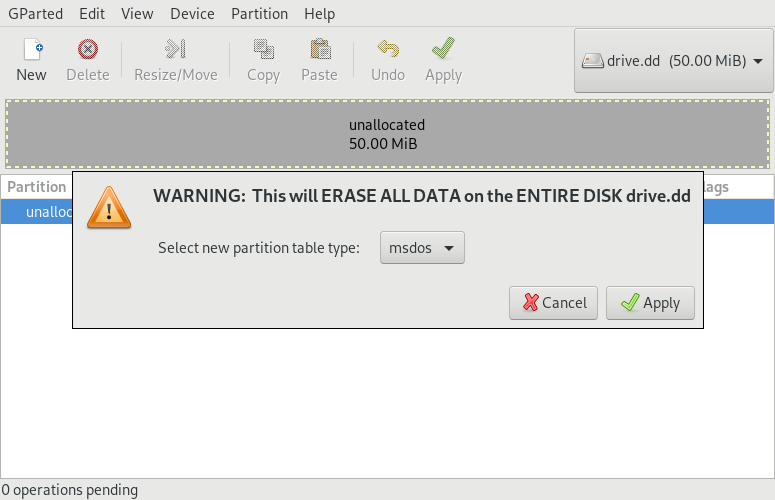
\includegraphics[scale=0.3]{images/tesi18.png}
 \caption[Gparted Partition Table]{ How to create a new partition table in Gparted.}
 \label{fig:gparted1}
    \end{center}
 \end{figure}

 \begin{figure}[h]
    \begin{center}
 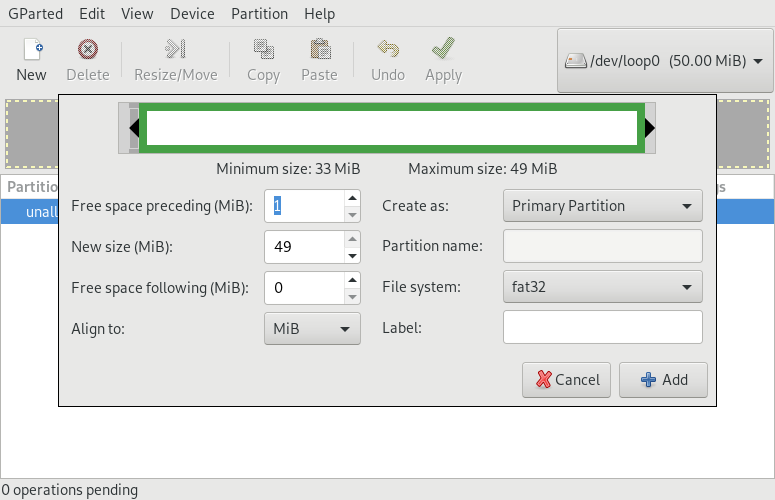
\includegraphics[scale=0.3]{images/tesi19.png}
 \caption[Gparted FAT32 Partition]{ How to create a new FAT32 partition in Gparted.}
 \label{fig:gparted2}
    \end{center}
 \end{figure}


After this the actual partitions can be written. Despite the microSD emulation, Qemu
does not follow the same boot process as a real Raspberry Pi 3; therefore, the 
disposition of partitions on disk and the presence of an actual {\tt kernel8.img}
binary on the first FAT32 partition is irrelevant. Nonetheless, MaldOS mimics the hardware 
restrictions and expects a single FAT32 partition. This configuration
step is depicted in figure \ref{fig:gparted2}.

Once everything is set the image file can be mounted and accessed again
through a loopback device. Note that, let {\tt /dev/loop0} be the associated 
loopback device, the actual partition to be mounted is different, probably in 
the form {\tt /dev/loop0p1}. All files copied into the image will be available 
for the emulated machine; tape and disk devices are added to MaldOS this way,
as files name {\tt TAPEn} and {\tt DISKn} (with \textit{n} ranging from 0 to 3),
respectively.\\

Another, perhaps faster method for achieving a suitable disk image consists in 
simply cloning a real disk (possibly a Raspberry Pi-ready microSD card) to a
binary file with the {\tt dd} tool, similarly to how the initial {\tt drive.dd}
was created:

\begin{lstlisting}[language=sh]
$ dd if=/dev/mmcblk0 of=drive.dd bs=1M
\end{lstlisting}

Where {\tt /dev/mmcblk0} is the disk device to be cloned.

\section{Debugging}
The debug of the compiled kernel can be carried over Qemu with GDB. Using the
{\tt -gdb tcp:1234} parameter Qemu opens a debugging tcp port for a GDB client
to connect to (another port can be specified). The {\tt -s} command line flag 
brings the same result in a shorter format, and by adding {\tt -S} as well the
emulator will not start the execution, allowing the developer to connect.

Once the emulator is ready, a GDB client can connect to it. A client for
ARM64 should be present within the toolchain used to compile the kernel.
 A simple command line client may attach using the following commands (assuming
 the {\tt aarch64-elf-gcc} toolchain is installed)

\begin{lstlisting}[label={lst:gdb}]
$ aarch64-elf-gdb
(gdb) file output.elf
(gdb) target remote localhost:1234
\end{lstlisting}

This GDB initial configuration can be added to a {\tt .gdbinit}
file for convenience to get automatically executed every time the debugger is run.\\

Emulators like $\mu$MPS2 have the prominent advantage of a specifically designed
running and debugging interface; nonetheless, a GDB server is a complete and
advanced debugging suite. The command line debugger may seem a scarce alternative,
but there are plenty of richer options; the author recommends {\tt gdbgui}, 
a browser-based Python GDB client.
Gdbgui can be installed via {\tt pip} or as an official package, depending on 
the Linux distribution. It must be launched
with the {\tt --gdb} (or {\tt -g}) command line option to specify a proper GDB
client (i.e. the one found within the ARM64 toochain); it acts as a web server
reachable at the default port {\tt 5000} with any browser, and provides an intuitive
interface fitted with step-by-step debugging, memory inspection, threaded view and
so on.
A {\tt .gdbinit} becomes especially useful when using Gdbgui as it is read even 
when the debugger is executed through the Python wrapper.

\subsection{Memory Management Unit}
Special care should be taken when debugging with the MMU enabled. To accomodate
virtual memory with ease of usage, the kernel image is loaded in physical address
space and virtualized only later. As has already been explained, this is a somewhat
uncharacteristic behaviour for a kernel, so support is not perfect.
When MMU is enabled the entry point for interrupt handlers in the form of the
\textbf{VBAR} register is shifted at address {\tt 0xFFFF000000000000}; the rest
of the kernel only uses relative references, so everything works.
However if the user is debugging the kernel he or she will become unable to break
execution on kernel code; logically, having moved all addresses 16 ExbiBytes forward
GDB will have a hard time finding symbols. To fix references again one must
load the elf symbol table with the same offset, using the following GDB command:

\begin{lstlisting}
(gdb) add-symbol-file output.elf 0xffff000000000000
\end{lstlisting}

Note that this directive too can be added to {\tt .gdbinit}. There is no 
obvious drawback to loading the symbol table at two separate offsets (the first
one being {\tt 0x0}); this way breakpoints will work regardless of the MMU state.


 \begin{figure}[t]
 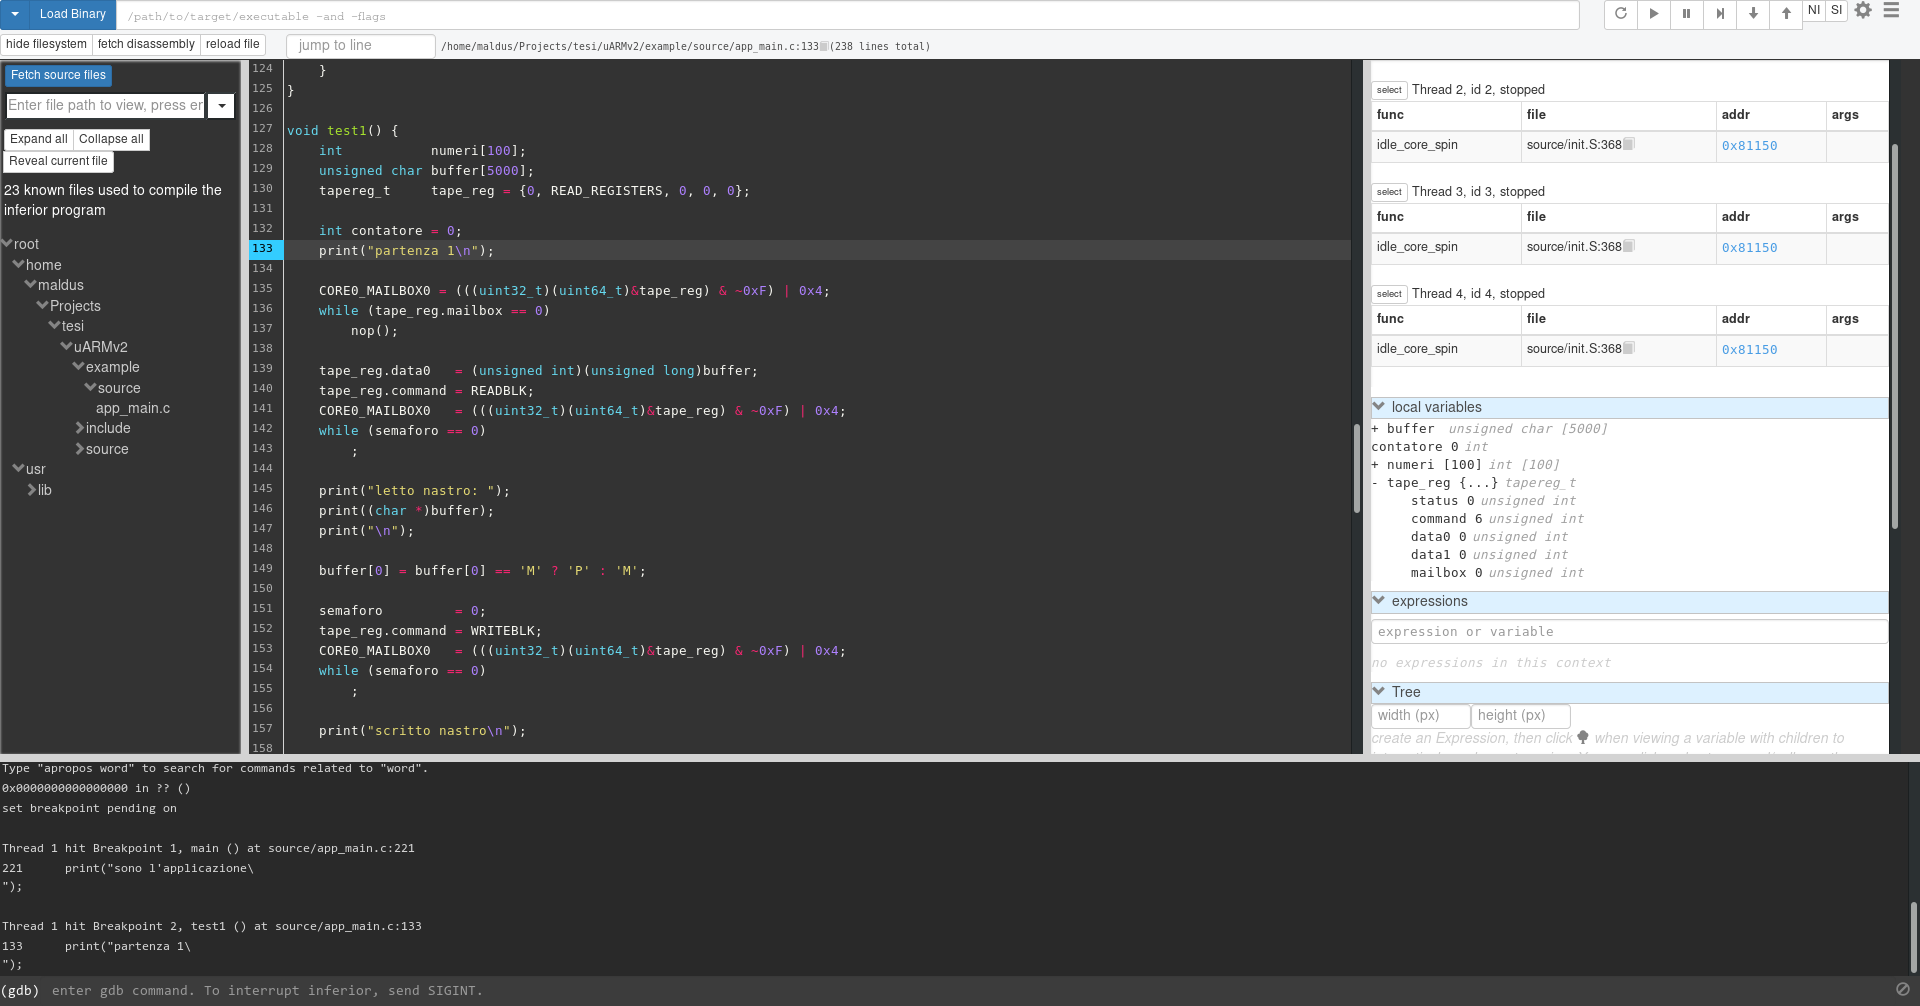
\includegraphics[scale=0.34,angle=-90,origin=c]{images/tesi4.png}
 \caption[Gdbgui]{gdbgui browser interface}\label{fig:gdbgui}
 \end{figure}





%%%%%%%%%%%%%%%%%%%%%%%%%%%%%%%%%%%%%%%%%non numera l'ultima pagina sinistra
\clearpage{\pagestyle{empty}\cleardoublepage}
%%%%%%%%%%%%%%%%%%%%%%%%%%%%%%%%%%%%%%%%%per fare le conclusioni
\chapter{Conclusions and Future Work}
\section{Extending Qemu}
The recently added Raspberry Pi machine configuration for Qemu only supports a few
capabilities of the original board: the two serial interfaces, the framebuffer
display and the microSD card EMMC.
The biggest missing part is of course the USB controller (bringing around the
Network interface as well); the base complexity of the USB protocol, however,
 would probably make it an unsuitable choice for learning projects anyway.

Peripherals of less practical value in an emulator would perhaps end up being
most interesting in the scope of OS study. SPI and I2C are relatively
easy low level serial protocols that could make an interesting addition to the
learning program; same goes for the PCM audio interface and the whole GPIO 
header in general.
Qemu is a fairly flexible emulator, and a future improvement could focus on 
enriching the virtual environment with more device options.

There is another consideration which has been ignored for the purposes of this
work: Qemu exists to virtualize generic machines for any architecture. The 
Raspberry Pi is a premium choice when the objective is learning, 
but an entirely new and ad-hoc virtual machine could be created and run on the
emulator just like $\mu$MPS2 does, only with the advantage of a widespread and
general purpose tool as backend. One could implement printers, terminals, disks,
tapes and even network interfaces not just as peripherals emulated by the abstraction
layer (which is somewhat redundant in a virtualized machine) but by the Qemu
emulator itself. \\
Moving away from ad-hoc tools in favor of Qemu is still an improvement
in the author's perspective, even though this obviously drops the advantage 
of running on real hardware as well.
However, on a more ambitious and visionary note, would it really? FPGA technology
has become more and more affordable in recent years, and with a stretch of imagination
the near future could harbor a FPGA board popularized like the Raspberry Pi and
capable of being programmed as an ARMv8 (or other, like RISC V) core. In this scenario the acts of 
building a new virtual Qemu machine and a real FPGA-hosted SoC would overlap,
allowing for a completely controlled real \textbf{and} virtual learning environment.\\
This is an arguably possible but very wild speculation.


\section{Debugging with GDB}
Being a off-the-shelf software GDB is flexible enough to be extended with 
a specifically tailored client. GDB provides a machine interpreter that recognizes
machine readable commands for the purpose of creating higher level interfaces.

If the generic approach of Gdbgui was deemed too complex for inexperienced graduate
students one could implement a $\mu$MPS2-like debugging interface that connects
to the Qemu GDB server. 
Following a more common approach for debuggers, a GDB compliant
 environment could be created inside a widely spread, extensible IDE like Atom or 
Visual Studio Code.\\
Indeed, by using generic GDB interface extensions it is already possible to debug
Qemu from VS Code. To improve on this it would suffice to add debugging widgets
with specific register and device views.

\section{Other ARM64 SoC}
Although it is now firmly seated in the Olympus of open source educational boards,
the Raspberry Pi family is build on awfully obscured and undocumented hardware.
Broadcom follows the market trend of not releasing any information on its 
products like other manufacturers.\\

There are many Raspberry Pi-like boards that base themselves on similar hardware
(namely, a powerful ARM CPU assisted by a graphical processing unit). In principle,
the work that has been done for the British board could be easily ported to a 
wide number of similar devices. For example Pine64, an open source family of products
taking heavy inspiration from the Raspberry Pi inheritance, has recently
marketed a laptop powered by one of their compute modules and is planning on 
a smartphone and tablet with the same characteristics. Running a toy
OS on a real-world mobile device could be both a more academically interesting 
exploit and an higher highlight for an undergraduate (or even graduate) student.

\section{Other Programming Languages}
Traditionally, Operating System kernels are written in C with critical parts
coded in Assembler. Some alternate higher level components using C-derived 
languages like C++ (Windows and Android) and Objective-C (IOS).
In the introduction some notable exceptions were mentioned: the Ultibo project 
\cite{ultibo} is a Raspberry Pi hardware abstraction layer written entirely in 
Pascal; Circle64 \cite{circle} is a similar library where C++ is used instead;
 when performance and resources are limited, one can find kernels written
entirely in Assembler (like KolibriOS).

Different programming languages obviously bring advantages and disadvantages,
but in the scope of educational work the choice falls unambigously on pure C.
It is the standard in Operating System development, and for good reasons:
simplicity, ease of carrying on low level memory operations, low portability 
dependencies, huge community and learning reference, perfect balance 
between abstraction and hardware fidelity.

Even beyond an academic objective, C is by far the dominant choice when it 
comes to kernel development and has been for decades. There is, however, a
contender that is recently emerging and gaining purchase thanks to its qualities
like performance, reliability and security: Rust.\\
Unlike the multitude of newly created programming languages of our time, Rust
has quickly managed to carve a spot in embedded development. As of now, it is 
already possible (and fairly easy) to run Rust code in various bare metal ARM
environment, Raspberry Pi included.

The main drawback lies in its inherent complexity: concepts like ownership and 
parallelism take a great deal of effort before mastery, and that would contrast
with the focus on OS development of this work. Nevertheless, Rust is considered
to be the closest second to C when it comes to the choice of programming language
and if it was included as an additional topic of study in future Computer Science
courses the opportunity should be considered seriously.

\section{Emulation Layer on Videocore IV}
Through the mailbox interface it is possible to ask the Broadcom GPU to directly
execute code: this is what happens with graphical firmware routines in fully
fledged Operating Systems like Raspbian.\\
In the early years code for the GPU was released only in binary form as proprietary 
software; only in 2012 Broadcom gave in and documented open source firmware for 
graphical processing. To this day a small component of proprietary binaries is 
still necessary to boot the Raspberry Pi (for example, {\tt bootcode.bin}), although
there are timid attempts at reverse engineering that as well.\\

If the Videocore IV was freely available for the developer like the ARM CPU, part
(if not the entirety) of the abstraction layer that is implemented as 
\textit{interrupt-in-the-middle} could be moved there. The interface to access
abstraction capabilities would not be much more convenient for the user, 
as the communication media would still be mailboxes; it would however provide
a more detailed emulation of hardware devices, for examble by acting as a real
DMA peripheral when reading and writing to emulated disks and tapes.
Students could write completely from scratch their Operating System, relying on 
GPU firmware to assist them in more complex tasks like device communication and
boot process.\\
It should be noted that this approach would probably break Qemu emulation, 
because the general purpose tool virtualizes the architecture, not the hardware.
There is no Videocore in the {\tt raspi3} machine: the kernel image is loading 
by Qemu and it is unclear to what degree mailboxes to the GPU respond correctly.

\section{Course Organization}
MaldOS was developed to be of assistance for students. The focus is on an Operating
Systems course, so effort was put into shaving off low level hardware interfacing
and initialization: the objective is to learn how an OS works, not the AArch64 Assembler
instruction set and registers, or how to operate the Arasan EMMC controller.\\
This approach however could be radically different depending on the subject under 
scrutiny. Low level Assembler programming and the ARM64 architecture are interesting
topics for a course in System Architectures. Given enough time, will and coordination,
the Kaya OS project could be build bottom-up by students in its entirety over four
semesters and two different courses: System Architectures for initialization and
peripheral interfacing and Operating Systems for the kernel and process management.

In that scenario, MaldOS is not a support for students anymore, but a mere example
and study on how to develop such an abstraction layer. Some sections would probably
end up identical even when created by other developers (there are few alterations
that can be made to the boot code, for example), but the interrupt handling in 
particular would become much less arbitrarily complicated. 

Overall, it would certainly be an extremely formative experience.

\begin{thebibliography}{90}             %crea l'ambiente bibliografia
\addcontentsline{toc}{chapter}{Bibliography}
%%%%%%%%%%%%%%%%%%%%%%%%%%%%%%%%%%%%%%%%%provare anche questo comando:
%%%%%%%%%%%\addcontentsline{toc}{chapter}{\numberline{}{Bibliografia}}
\bibitem{minix} Andrew S. Woodhull, Andrew S. Tanenbaum, 
                Operating System Design and Implementation, 1997.
\bibitem{bakingpi} University of Cambridge, Department of Computer Science and Technology,
                    Baking Pi - Operating Systems Development,
                    \url{https://www.cl.cam.ac.uk/projects/raspberrypi/tutorials/os/}
\bibitem{davolimorsiani} M. Goldweber, R. Davoli, and M. Morsiani,
                        \"The Kaya OS project and the $\mu$MPS hardware emulator\",
                          SIGCSE Bull., vol. 37, pp. 49-53, June 2005.
\bibitem{tesijonjic} T. Jonjic,
                    \"Design and Implementation of the $\mu$MPS2 Educational Emulator\",
                    Alma Mater Studiorum, 2012.
\bibitem{tesimelletti} M. Melletti,
                    \"Studio e Realizzazione dell'emulatore $\mu$ARM e del progetto
                    JaeOS per la Didattica dei Sistemi Operativi\",
                    Alma Mater Studiorum, 2016.
\bibitem{pop} M. Goldweber, R. Davoli, $\mu$MPS Principles of Operation, Lulu Books, 2011
\bibitem{raspberrypios} Raspberry Pi OS, \url{https://github.com/s-matyukevich/raspberry-pi-os}
\bibitem{ultibo} The Ultibo Project, \url{https://ultibo.org/}
\bibitem{circle} The Circle C++ environment, \url{https://github.com/rsta2/circle}
\bibitem{bcm2835} BCM2835 ARM Peripherals, Broadcom.
\bibitem{rev3.4} ARM Quad A7 Core, Broadcom.
\bibitem{pl011} PrimeCell UART (PL011) Technical Reference Manual, ARM.
\bibitem{guide} ARM Cortex-A Series Programmer's Guide for ARMv8-A, ARM, 2015.
\bibitem{armarm} ARM Architectural Reference Manual ARMv8, for ARMv8-A Architecture Profile, ARM, 2017.
\bibitem{a53} ARM Cortex-A53 MPCore Processor, ARM, 2016.
\end{thebibliography}
%%%%%%%%%%%%%%%%%%%%%%%%%%%%%%%%%%%%%%%%%non numera l'ultima pagina sinistra
\clearpage{\pagestyle{empty}\cleardoublepage}
\chapter*{Ringraziamenti}
\thispagestyle{empty}
Qui possiamo ringraziare il mondo intero!!!!!!!!!!\\
Ovviamente solo se uno vuole, non \`e obbligatorio.
\end{document}
